\title{Resumen de Fisica 3}

\author{Mateo P. Cetti}

\documentclass[10pt]{article}

\usepackage{amsmath}
\usepackage{amsfonts}
\usepackage{graphicx}

\begin{document} 
\maketitle

\section{Movimiento ondulatorio}

El mundo está lleno de \textbf{ondas}, los dos tipos principales son las ondas \textbf{mecánicas} 
(Tirar una piedra al agua) y las ondas \textbf{electromagnéticas} (las ondas de radio). En el caso de las 
ondas mecánicas, algunos medios físicos se perturban. Las ondas
electromagnéticas no requieren un medio para propagarse.\\
La caracteristica principal del movimiento ondulatorio es que la \textbf{energía} se 
transfiere a través de una distancia, perola \textbf{materia} no.

\paragraph{Ondas mecanicas}

Todas las ondas mecánicas requieren:

\begin{enumerate}
    \item alguna fuente de perturbación
    \item un medio que contenga elementos que sean factibles de perturbación
    \item algún mecanismo físico a partir del cual los elementos del medio puedan influirse mutuamente.
\end{enumerate}

\paragraph{Tipos de ondas: }

\begin{itemize}
    \item \textbf{onda transversal} Una onda viajera o pulso que hace que los elementos 
    del medio perturbado se muevan \textbf{perpendiculares} a la dirección de propagación.
    \item \textbf{onda longitudinal} Una onda viajera o pulso que mueve a los elementos del medio en \textbf{paralelo}
    a la dirección de propagación
\end{itemize}

\paragraph{Funcion de onda}
\begin{itemize}
    \item $y(x, t) y(x-vt, 0)$ (Si el pulso viaja hacia la \textbf{derecha} en X)
    \item $y(x, t) y(x+vt, 0)$ (Si el pulso viaja hacia la \textbf{izquierda} en X)
\end{itemize}

La función de onda y(x, t) representa la coordenada y, la posición transversal,
de cualquier \textbf{elemento} ubicado en la posición x en cualquier tiempo t.\\
\linebreak
Ademas, si t es fijo (como en el caso de tomar una instantánea del pulso), la función 
de onda y(x), a veces llamada \textbf{forma de onda}, define una curva que representa la 
\textbf{forma} geométrica del \textbf{pulso} en dicho tiempo.

\paragraph{El modelo de onda progresiva}

Primero, la forma de onda completa se mueve hacia la derecha de modo que la curva 
se mueve hacia la derecha y al final llega a la posición de la curva azul. Este es el \textbf{movimiento 
de la onda}. Si se concentra en un elemento del medio, como el elemento en x = 0, observará que cada
elemento se mueve hacia arriba y hacia abajo a lo largo del eje y en movimiento armónico
simple. Este es el \textbf{movimiento de los elementos del medio}. Es importante \textbf{diferenciar} entre el
movimiento de la onda y el movimiento de los elementos del medio.

\paragraph{modelo de onda}

Un punto en la figura en que el desplazamiento del elemento de su 
posición normal está más alto se llama \textbf{cresta} de la onda.\\

El punto más bajo se llama \textbf{valle}.\\

la longitud de onda ($\lambda$) es la \textbf{distancia mínima} entre dos puntos
cualesquiera en ondas adyacentes\\

\textbf{periodo} T de las ondas es el intervalo de tiempo requerido 
para que dos puntos idénticos de ondas adyacentes pasen por un punto.\\

\textbf{frecuencia} $f$ de una onda periódica es el número de crestas (o
valles o cualquier otro punto en la onda) que pasa un punto determinado en un intervalo
de tiempo \textbf{unitario}.\\

\begin{equation*}
    f = \dfrac{1}{T}
\end{equation*}

La \textbf{máxima posición} de un elemento del medio relativo a su \textbf{posición de equilibrio} se
llama \textbf{amplitud} A de la onda.\\

Las ondas viajan con una \textbf{rapidez} específica, y esta rapidez depende de las \textbf{propiedades
del medio perturbado}.\\

\paragraph{Formas de la funcion de onda:}
Forma 1:
\begin{equation*}
    y(x, t) =  A sen \left[ \frac{2\pi}{\lambda} (x-vt) \right] 
\end{equation*}

$v = \dfrac{\lambda}{T}$. Sustituyendo esto en la ecuacion anterior:

\begin{equation*}
    y = Asen \left[ 2\pi \left( \frac{x}{\lambda} - \frac{t}{T} \right) \right] 
\end{equation*}

Para abreviar la formula definimos:\\
\linebreak

\textbf{número de onda angular: }$k = \dfrac{2\pi}{\lambda}$

\textbf{frecuencia angular: }$w = \dfrac{2\pi}{T} = 2\pi f$\\
\linebreak
Entonces la funcion queda:

\begin{equation*}
    y = Asen(kx-wt)
\end{equation*}

Ademas, $v$ se puede definir alternativamente como: $v = \frac{w}{f} = \lambda f$\\
\linebreak
La función de onda conocida en la ecuación supone que la posición vertical y de
un elemento del medio es cero en $x=0$ y $t=0$. Este no necesita ser el caso. Si no lo es, la
función de onda por lo general se expresa en la forma:\\
$y = Asen(kx-wt + \phi)$\\
donde $\phi$ es la \textbf{constante de fase}

\paragraph{Ondas sinusoiodales en cuerdas}

Se puede usar esta expresión para describir el movimiento de cualquier elemento de la
cuerda. Un elemento en el punto P se mueve sólo verticalmente, y de este modo su coordenada x 
permanece constante. Por lo tanto, la rapidez transversal $v_y$ (no confundir con la 
rapidez de onda v) y la aceleración transversal $a_y$ de los \textbf{elementos} de la cuerda son

\begin{equation*}
    v_y = -wA cos(kx-wt)
\end{equation*}

\begin{equation*}
    a_y = -w^2 A sen(kx-wt)
\end{equation*}

Los valores \textbf{máximos} de la rapidez transversal y la
aceleración transversal son simplemente los valores absolutos de los coeficientes de las
funciones coseno y seno:

\begin{equation*}
    v_y max = wA
\end{equation*}

\begin{equation*}
    a_y max = w^2 A
\end{equation*}

La \textbf{rapidez transversal} y la \textbf{aceleración transversal} de los elementos de la cuerda no llegan
\textbf{simultáneamente} a sus valores máximos. La rapidez transversal llega a su valor máximo
($wA$) cuando $y=0$, mientras que la magnitud de la aceleración transversal llega a su valor
máximo ($w^2A$) cuando $y= \pm A$

\paragraph{La rapidez de ondas en cuerdas}

En esta sección se determina la rapidez de un pulso transversal que viaja en una cuerda
tensa. Primero cabe mencionar que se espera que la \textbf{rapidez} de la onda \textbf{aumente} con una
\textbf{tensión creciente} y debe disminuir a medida que \textbf{aumente} la \textbf{masa por unidad de longitud} 
de la cuerda.\\
\linebreak
Si la tensión en la cuerda es $T$ y su masa por unidad
de longitud es $\mu$, la rapidez de onda es:

\begin{equation*}
    \sqrt{\dfrac{T}{\mu}}
\end{equation*}

\paragraph{Reflexión y transmisión}

El modelo de onda progresiva describe ondas que viajan a través de un medio uniforme sin
interactuar con algo más en el camino. Ahora se considerará cómo una onda progresiva
es afectada cuando \textbf{encuentra un cambio} en el medio\\
\linebreak
considere un pulso que viaja en una cuerda que está rígidamente unida a un soporte en un extremo, como en
la figura. Cuando el pulso alcanza el soporte, se presenta un cambio severo en el medio: la
cuerda termina. Como resultado, el pulso experimenta reflexión; es decir, el pulso se
mueve de regreso a lo largo de la cuerda en la dirección opuesta.Note que el pulso reflejado está invertido.\\
\linebreak
Ahora considere otro caso. Esta vez, el pulso llega al final de una cuerda que es libre
de moverse verticalmente, como en la figura 16.14. La tensión en el extremo libre se mantiene porque la cuerda está amarrada a un anillo de masa despreciable que tiene libertad
para deslizarse verticalmente sobre un poste uniforme sin fricción. De nuevo, el pulso
se refleja, pero esta vez no se invierte. \\
\linebreak
Para finalizar, considere una situación en la que la frontera es intermedia entre estos
dos extremos. En este caso, parte de la energía en el pulso incidente se refleja y parte se
somete a transmisión; es decir: parte de la energía pasa a través de la frontera. Por ejemplo, 
suponga que una cuerda ligera se une a una cuerda más pesada,

\paragraph{Rapidez de transferencia de energía mediante ondas sinusoidales
en cuerdas}

La energía cinética de un elemento de la cuerda se expresa como: 
\begin{equation*}
    dK = \frac{1}{2} (\mu dx) v_y^2
\end{equation*}

Al sustituir con la ecuación para la rapidez transversal general 
de un oscilador armónico simple se obtiene:

\begin{equation*}
    dK = \frac{1}{2} \mu w^2 A^2 cos^2 (kx-wt) dx 
\end{equation*}

Si se toma una instantánea de la onda en el tiempo t=0, la energía cinética de un elemento dado es:

\begin{equation*}
    dK = \frac{1}{2} \mu w^2 A^2 cos^2 (kx) dx 
\end{equation*}

Al integrar esta expresión sobre todos los elementos de cuerda en una longitud de onda
de la onda produce la energía cinética total KA en una longitud de onda:

\begin{equation*}
    dK_\lambda = \frac{1}{4} \mu w^2 A^2 \lambda 
\end{equation*}

para la energía potencial total $U_A$
en una longitud de onda produce exactamente el mismo resultado:

\begin{equation*}
    dU_\lambda = \frac{1}{4} \mu w^2 A^2 \lambda 
\end{equation*}

La energía total en una longitud de onda de la onda es la suma de las energías potencial
y cinética:

\begin{equation*}
    E_\lambda = U_\lambda + K_\lambda =  \frac{1}{4} \mu w^2 A^2 \lambda 
\end{equation*}

Por lo tanto, la potencia $\mathbb{P}$, o rapidez de transferencia de energía $T_{OM}$ asociada
con la onda mecánica, es

\begin{equation*}
    \mathbb{P} = \frac{1}{2} \mu w^2 A^2 v
\end{equation*}

\paragraph{La ecuación de onda lineal}

Todas las funciones de onda y(x, t) representan soluciones de
una ecuación llamada ecuación de onda lineal. Esta es:

\begin{equation*}
	\dfrac{\partial^{2} y}{\partial x^2} = \dfrac{1}{v^2} \dfrac{\partial^2 y}{\partial t^2}
\end{equation*}

\section{Ondas sonoras}
Las \textbf{sonoras} viajan a través de \textbf{cualquier } medio material con una rapidez que depende
de las \textbf{propiedades del medio}.\\
\linebreak
A medida que las ondas sonoras viajan a través del aire, los
elementos del aire \textbf{vibran} para producir cambios en \textbf{densidad} y \textbf{presión} a lo largo de la
dirección del movimiento de la onda.\\ 
\linebreak
Si la fuente de las ondas sonoras vibra sinusoidalmente, las variaciones de presión también son sinusoidales.\\
\linebreak
Las ondas sonoras se dividen en \textbf{tres categorías} que cubren diferentes intervalos de frecuencia.\\ 
\begin{enumerate}
	\item Las \textbf{ondas audibles} se encuentran dentro del intervalo de sensibilidad del oído
		humano.
	\item Las \textbf{ondas infrasónicas} tienen frecuencias por abajo del
		intervalo audible.
	\item Las \textbf{ondas ultrasónicas} tienen frecuencias por arriba del alcance audible.
\end{enumerate}

\paragraph{Rapidez de ondas sonoras}

Un pistón en el extremo izquierdo se mueve hacia la derecha para \textbf{comprimir el gas} y crear el pulso.
Antes de que el pistón se mueva, el gas \textbf{no está perturbado} y tiene \textbf{densidad uniforme},
cuando el pistón se empuja súbitamente hacia la derecha, el gas justo \textbf{enfrente} de él se \textbf{comprime};
la presión y la densidad en esta región ahora son mayores de lo que eran antes de que el
pistón se moviera. Cuando el pistón \textbf{se detiene}, la región comprimida del
gas \textbf{continúa en movimiento} hacia la derecha, lo que corresponde a un \textbf{pulso longitudinal}
que viaja a través del tubo con rapidez $v$.\\
\linebreak
La \textbf{rapidez} de las ondas sonoras en un medio depende de la \textbf{compresibilidad} y la \textbf{densidad} del medio; si éste es un \textbf{líquido} o un \textbf{gas} y tiene un módulo volumétrico B y densidad $p$, la rapidez de las ondas sonoras en dicho medio es

\begin{equation*}
	v = \sqrt[2]{\dfrac{B}{p}}
\end{equation*}

La rapidez del sonido también depende de la \textbf{temperatura} del medio. La relación entre
la rapidez de la onda y la temperatura del aire, para sonido que viaja a través del aire, es:

\begin{equation*}
	v = (331 m/s) \sqrt{1+\frac{T_c}{273ºC}}
\end{equation*}

Donde 331 m/s es la rapidez del sonido en aire a 0°C y $T_c$ es la \textbf{temperatura} del aire en grados celsius.

\paragraph{Ondas sonoras periódicas}
Una región comprimida se forma siempre que el pistón se empuje
en el tubo. Esta región comprimida, llamada \textbf{compresión}, se mueve a través del tubo, y
comprime continuamente la región justo enfrente de ella misma.\\
\linebreak
Cuando el pistón se jala hacia atrás, el gas enfrente de él se expande y la presión y la densidad en esta región caen
por abajo de sus valores de equilibrio. Estas regiones de baja presión, llamadas \textbf{enrarecimiento},
también se propagan a lo largo del tubo, siguiendo las compresiones.\\
A medida que el pistón tiene una oscilación sinusoidal, se establecen continuamente
regiones de compresión y enrarecimiento.\\
\linebreak 
La distancia entre dos compresiones sucesivas (o dos enrarecimientos sucesivos) iguala 
la \textbf{longitud de onda} $\lambda$ de la onda sonora.\\
\linebreak
Mientras estas regiones viajan a través del tubo, cualquier elemento pequeño del medio se mueve
con movimiento \textbf{armónico simple paralelo} a la dirección de la onda.\\
\linebreak
Si $s(x, t)$ es la posición de un elemento pequeño en relación con su posición de equilibrio,
 se puede expresar esta función de posición armónica como:
\begin{equation*}
 	s(x,t) = s_{max} \cos(kx-wt)
\end{equation*}

Donde $s_{max}$ es la posicion maxima del elemento relativo al equilibrio y se denomina \textbf{Amplitud de desplazamiento}.
( el desplazamiento del elemento es a lo largo de $x$)

La variación en la presión del gas $\Delta P$ observada desde el valor de equilibrio también es
periódica. $\Delta P$ se conoce por:

\begin{equation*}
 	\Delta p(x,t) = \Delta p_{max} \cos(kx-wt)
\end{equation*}

donde la amplitud de presión $\Delta p_{max}$, que es el \textbf{cambio máximo en presión} desde el valor
de equilibrio, se proporciona por

\begin{equation*}
	\Delta p_{max} = pvws_{max}
\end{equation*}

La variación de presión es un \textbf{máximo} cuando el desplazamiento
desde el equilibrio es \textbf{cero}, y el desplazamiento desde el equilibrio es un \textbf{máximo} cuando
la variación de presión es \textbf{cero}.

\paragraph{Intensidad de ondas sonoras periódicas}

se demostró que una onda que viaja sobre una cuerda tensa transporta
energía. Se aplica el mismo concepto a ondas sonoras. La energía cinética en una longitud de onda de
la onda sonora es

\begin{equation*}
	K_{\lambda} = \frac{1}{4} (pA)w^2s^2_{max}\lambda	
\end{equation*}

la \textbf{energía mecánica} total para una longitud de onda es

\begin{equation*}
	E_{\lambda} = K_{\lambda} + U_{\lambda}  = \frac{1}{2} (pA)w^2s^2_{max}\lambda
\end{equation*}

la rapidez de transferencia de energía es

\begin{equation*}
	P = \frac{1}{2} pAvw^2s^2_{max}\lambda
\end{equation*}

donde $v$ es la rapidez del sonido en el aire.

La \textbf{intensidad} $I$ de una onda, se define como la
\textbf{rapidez} a la cual la energía transportada por la onda se transfiere a través de una unidad
de área A \textbf{perpendicular} a la dirección de viaje de la onda:

\begin{equation*}
	I = \dfrac{P}{A}
\end{equation*}

\begin{equation*}
	I = \dfrac{1}{2} pv(ws_{max})^2
\end{equation*}

\begin{equation*}
	I = \dfrac{(\Delta P_{max})^2}{2pv}
\end{equation*}

Cuando una fuente emite sonido por igual en todas
direcciones, el resultado es una \textbf{onda esférica}.\\
Cada arco representa
una superficie sobre la cual es constante la fase de la onda. A tal superficie 
de fase constante se le llama \textbf{frente de onda}.\\
Las líneas radiales que se dirigen hacia
afuera desde la fuente se llaman \textbf{rayos}.\\
\linebreak
La potencia promedio $P_{prom}$ emitida por la fuente debe tener una distribución uniforme sobre cada frente de onda esférica de área. Por tanto, la intensidad de la onda a
una distancia $r$ de la fuente es

\begin{equation*}
	I = \dfrac{P_{prom}}{4\pi r^2}
\end{equation*}

\paragraph{Nivel sonoro en decibeles}

El nivel sonoro $\beta$ se define mediante la ecuación

\begin{equation*}
	\beta = 10 \log \left( \dfrac{I}{I_0} \right)
\end{equation*}

La constante $I_0$ es la \textbf{intensidad de referencia}, considerada como el umbral de audición
($I_0 = 1 * 10^{-12}$ W/$m^2$) $I$ es la intensidad en watts por cada metro cuadrado a la 
que corresponde el nivel de sonido $\beta$, donde $\beta$ se mide en decibeles (dB).

\paragraph{El efecto Doppler}

Tal vez haya notado cómo \textbf{varía el sonido} del claxon de un vehículo a medida que éste
se aleja. La \textbf{frecuencia} del sonido que escucha mientras el vehículo se aproxima a usted es
\textbf{más alta} que la frecuencia que escucha mientras se aleja. Esta experiencia es un ejemplo
del \textbf{efecto Doppler}.\\
\linebreak

Sean $f$ la frecuencia de la fuente, $\lambda$ la longitud de onda y $v$ la rapidez del sonido en
la figura Si el observador también queda estable, detectará frentes de onda a una frecuencia $f$.
Cuando el observador se mueve \textbf{hacia} la fuente, la rapidez de las ondas
relativa al observador es $v' = v + v_0$, pero la
longitud de onda $\lambda$ no cambia. Se puede decir
que la frecuencia $f$ que escucha el observador está \textbf{aumentada} y se conoce por
\begin{equation*}
	f' = \dfrac{v'}{\lambda} = \dfrac{v+v_0}{\lambda}
\end{equation*}
Ya que $\lambda = v/f$, $f'$ se puede expresar como:
\begin{equation*}
	f' = \left( \dfrac{v+v_0}{\lambda}  \right)f
\end{equation*}

Si el observador es móvil alejándose de la fuente, la rapidez de la onda 
relativa al observador es $v' = v-v_0$. En este caso la frecuencia escuchada por el observador queda \textbf{reducida}
y se encuentra por:

\begin{equation*}
	f' = \left( \dfrac{v-v_0}{\lambda}  \right)f
\end{equation*}


Ahora suponga que la \textbf{fuente} está en movimiento y que el observador queda en reposo.\\
Si la fuente avanza directo hacia el observador, los \textbf{frentes de onda} escuchados por el observador están más juntos de lo que estarían si la fuente no se moviera.


Como resultado, la longitud de onda $\lambda$ medida por el observador es mas corta que la
longitud de onda $\lambda$ de la fuente. Durante cada vibración, que dura un intervalo de tiempo
$T$ (el periodo), la fuente se mueve una distancia $v_sT = \frac{v_s}{f}$ y la longitud de onda se \textbf{acorta}
en esta cantidad. Por lo tanto, la longitud de onda observada $\lambda'$ es:

\begin{equation*}
	\lambda' = \lambda - \Delta \lambda = \lambda - \dfrac{v_s}{f}
\end{equation*}


Como $\lambda = v/f$, la frecuencia $f$ que escucha el observador es:

\begin{equation*}
	f' = \dfrac{v}{(v/f)-(v_s/f)}	
\end{equation*}

La frecuencia observada aumenta siempre que la fuente se mueva hacia el observador.

\begin{equation*}
	f' = \left( \dfrac{v}{v-v_s}\right)f
\end{equation*}
La frecuencia observada disminuye siempre que la fuente se aleje del observador:
\begin{equation*}
	f' = \left( \dfrac{v}{v+v_s}\right)f
\end{equation*}

Por último, al combinar las ecuaciones se obtiene la siguiente correspondencia general para la frecuencia observada:

\begin{equation*}
	f' = \left( \dfrac{v \pm v_0}{v \pm v_s}\right)f
\end{equation*}

\pagebreak

\section{Sobreposición e interferencia}

\textbf{Principio de sobrepocicion: } Si dos o más ondas progresivas se mueven a través de un medio, el valor resultante
de la función de onda en cualquier punto es la suma algebraica de los valores de las
funciones de onda de las ondas individuales.\\
\linebreak
Las ondas que obedecen este principio se llaman \textbf{ondas lineales} (tienen amplitudes mucho menores
que sus longitudes de onda).\\
\linebreak
Las ondas que violan el principio de sobreposición se llaman
ondas \textbf{no lineales} y con frecuencia se caracterizan por grandes amplitudes.\\
\linebreak
Una consecuencia del principio de sobreposición es que dos ondas progresivas pueden
pasar una a través de la otra sin \textbf{alterarse}\\
\linebreak
La función de onda para el pulso móvil hacia la derecha es $y_1$, y la función de onda para el
pulso móvil hacia la izquierda es $y_2$. Cuando las ondas comienzan a traslaparse, la función de
onda para la onda compleja resultante se conoce por $y_1+y_2$. Cuando las crestas de los
pulsos \textbf{coinciden}, tiene una \textbf{amplitud} 
mayor que los pulsos individuales. Los dos pulsos finalmente se separan y \textbf{continúan}
su movimiento en sus direcciones originales.\\
\linebreak
La combinación de ondas separadas en la misma región de espacio para producir una
onda resultante se llama \textbf{interferencia}.\\
\linebreak
Cuando los desplazamientos causados por los dos pulsos están en la \textbf{misma dirección}, a esta interferencia se le
refiere como \textbf{interferencia constructiva}.\\
\linebreak
Cuando los desplazamientos causados por los dos pulsos están en direcciones
\textbf{opuestas}, a su superposición se le refiere como \textbf{interferencia destructiva}.\\
\linebreak
\paragraph{Sobreposición de ondas sinusoidales}
Si las dos ondas viajan hacia la derecha y tienen
la misma frecuencia, longitud de onda y amplitud pero difieren en fase, sus funciones de
onda individuales se pueden expresar como:
\begin{equation*}
	y = 2Acos\left( \dfrac{\phi}{2} \right)sen\left( kx-wt+  \dfrac{\phi}{2} \right)
\end{equation*}
La función de onda resultante y
también es \textbf{sinusoidal} y tiene la misma \textbf{frecuencia} y \textbf{longitud de onda}
 que las ondas individuales.\\
La amplitud de la onda resultante es $2Acos\left( \dfrac{\phi}{2} \right)$  y su fase
es $\dfrac{\phi}{2}$.\\
Si la constante de fase $\phi$ igual a 0 ($cos(0) = 1$) la amplitud de onda resultante es igual a $2A$. En
este caso, se dice que las ondas están \textbf{en fase}.\\
\linebreak
Cuando $\phi$ es igual a $\pi$ radianes o a cualquier múltiplo impar de $\pi$, y las crestas de una onda se presentan en las mismas posiciones que los valles de la segunda (\textbf{interferencia destructiva})  la onda resultante tiene amplitud \textbf{cero} en todas partes.\\
\linebreak
En último lugar, cuando la constante de fase tiene un valor arbitrario distinto de 0 o un múltiplo entero de
$\pi$ radianes, la onda resultante tiene una amplitud cuyo valor está en alguna
parte entre 0 y 2A.\\

\paragraph{Interferencia de ondas sonoras}.\\
\textbf{Longitud de trayectoria}($r$) La distancia a lo largo de cualquier
trayectoria de la bocina al receptor\\
Se puede dar el caso en el que desde una bocina hasta al receptor haya 2 trayectorias.\\
Cuando la diferencia en las longitudes de trayectoria $\Delta r = |r_2-r_1|$ es $0$ o algun 
multiplo entero de $\lambda$ ($\Delta r = n\lambda \rightarrow n = 0,1,2,3,...$), ), las dos ondas que 
llegan al receptor en cualquier instante están en fase y se interfieren \textbf{constructivamente} ( se detecta un máximo en la intensidad sonora).\\
\linebreak
Si $r_2$ es tal que $\Delta r = |r_2-r_1| = \dfrac{\lambda}{2}, 3\dfrac{\lambda}{2}, n\dfrac{\lambda}{2} $  las dos ondas están exactamente $\pi$ radianes, fuera de fase en el receptor y por tanto se cancelan mutuamente (no se detecta sonido).

\paragraph{Ondas estacionarias}
Se consideran funciones de onda para dos ondas sinusoidales transversales que tengan la misma amplitud, frecuencia y longitud de onda pero que viajen en direcciones opuestas en el mismo medio
\begin{equation*}
	y = 2Asen(kx)cos(wt)
\end{equation*}

Esta es la funcion de una \textbf{onda estacionaria}. Es un patrón de oscilación con un contorno 
estacionario que resulta de la sobreposición de dos ondas \textbf{idénticas}
que viajan en direcciones \textbf{opuestas} ( no es
una expresión para \textbf{una sola} onda progresiva).\\
no hay sentido de movimiento en la dirección de propagación de cualquier onda
original.\\
Cada elemento del medio oscila en movimiento armónico con la misma frecuencia angular $w$.\\
Sin embargo, la amplitud del movimiento armónico simple de un elemento depende de la ubicación
$x$ del elemento en el medio.\\
La amplitud del movimiento armónico simple de un elemento del medio tiene un valor
mínimo de \textbf{cero} cuando x satisface la condición sen $kx= 0$.($kx = 0, \pi, 2\pi$).\\
Como $k = 2\pi/\lambda$, estos valores para $kx$ producen:
\begin{equation*}
	x = 0, \frac{\lambda}{2}, \lambda, \frac{3\lambda}{2}, \frac{n\lambda}{2} \rightarrow n=0,1,2,3,4,5,...
\end{equation*}

Estos puntos de amplitud cero se llaman \textbf{nodos}.\\
\linebreak
El elemento del medio con el \textbf{mayor} desplazamiento posible desde el equilibrio tiene
una amplitud de 2A. Las posiciones en el medio donde se presenta este desplazamiento máximo se llaman \textbf{antinodos}. Los
antinodos se ubican en posiciones que satisfacen la condición $sen kx= \pm1$ de la coordenada x, es decir, cuando:
\begin{equation*}
	kx =  \dfrac{\pi}{2},  \dfrac{3\pi}{2},  \dfrac{5\pi}{2}
\end{equation*}
Por lo tanto, las posiciones de los antinodos se dan por:
\begin{equation*}
	x = \dfrac{n\lambda}{4} \rightarrow n = 1,3,5,...
\end{equation*}

La distancia entre \textbf{antinodos} adyacentes es igual a $\lambda/2$.\\
La distancia entre \textbf{nodos} adyacentes es igual a $\lambda$/2.\\
La distancia entre un \textbf{nodo} y un \textbf{antinodo} adyacente es $\lambda$/4.\\

\paragraph{Ondas estacionarias en una cuerda fija
en ambos extremos}

En una cuerda se pueden establecer \textbf{ondas estacionarias} mediante una \textbf{sobreposición} continua de ondas
\textbf{incidentes} y \textbf{reflejadas} desde los extremos. Pero hay una \textbf{condicion frontera}: Los extremos de la cuerda (al estar fijos) son \textbf{nodos} por definicion.\\
\linebreak
Esta condición frontera resulta en que la cuerda tenga un número de 
patrones de oscilación naturales discretos, llamados \textbf{modos normales}.\\
La sección de una onda estacionaria de un nodo al siguiente se llama \textbf{bucle}\\
\linebreak
El primer modo normal tiene nodos en sus extremos y un antinodo en medio (un solo bucle). En este caso,
la longitud de onda $\lambda_1$ es igual al doble de la longitud de la cuerda ($\lambda_1 = 2L$)\\
\linebreak
El segundo modo normal es cuando $\lambda_2 = L$ (2 bucles).\\
\linebreak
El tercer modo normal es cuando $\lambda_3 = \dfrac{2L}{3}$ (3 bucles).\\
\linebreak
En general, las
longitudes de onda de los diferentes modos normales para una cuerda de longitud L fija
en ambos extremos son:
\begin{equation*}
	\lambda_n = \dfrac{2L}{n} \rightarrow n = 1,2,3,...
\end{equation*}

 las frecuencias naturales $f_n$ de los modos normales son
\begin{equation*}
	f_n = \dfrac{v}{\lambda_n} = n\dfrac{v}{2L} = \dfrac{n}{2L} \sqrt{\dfrac{T}{\mu}} \rightarrow n = 1,2,3,...
\end{equation*}
La frecuencia más baja de todas, $f_1$, que corresponde a $n = 1$, se llama \textbf{frecuencia fundamental } 
y se conoce por:
\begin{equation*}
	f_1 =  \dfrac{1}{2L} \sqrt{\dfrac{T}{\mu}}
\end{equation*}

\paragraph{Resonancia}
Se vio que un sistema como una cuerda tensa es capaz de oscilar en uno o más modos
de oscilación normales. Si una fuerza periódica se aplica a tal sistema, la amplitud del
movimiento resultante es mayor cuando la frecuencia de la fuerza aplicada es \textbf{igual} a una
de las \textbf{frecuencias naturales} del sistema. Este fenómeno, conocido como \textbf{resonancia}\\
\linebreak
Ya que un sistema en oscilación muestra una gran amplitud cuando se activa a cualquiera de sus
frecuencias naturales, a estas frecuencias por lo general se les refiere como \textbf{frecuencias
de resonancia}.

\paragraph{Ondas estacionarias en columnas de aire}
El modelo de ondas bajo condiciones frontera también se aplica a ondas sonoras en una
columna de aire. Las ondas estacionarias son resultado de la interferencia entre ondas sonoras longitudinales que
viajan en direcciones opuestas.\\
\begin{itemize}
	\item \textbf{tubo cerrado en un extremo} dicho extremo es un \textbf{nodo} de desplazamiento y un  un \textbf{antinodo} de
presión.
	\item \textbf{Tubo abierto en ambos extremos} El extremo abierto de una columna de aire es aproximadamente un \textbf{antinodo} de desplazamiento y un \textbf{nodo} de presión
\end{itemize}

Las columnas de aire tienen \textbf{frecuencias cuantizadas}.
\begin{center}
	En un tubo abierto en ambos extremos, las frecuencias naturales de oscilación forman una serie armónica que incluye todos los múltiplos enteros de la frecuencia
fundamental.
\end{center}

\begin{equation*}
	f_n = n\dfrac{v}{2L} \rightarrow n = 1,2,3,...
\end{equation*}

\begin{center}
	En un tubo cerrado en un extremo, las frecuencias de oscilación naturales forman
una serie armónica que incluye sólo múltiplos enteros impares de la frecuencia
fundamental.
\end{center}

\begin{equation*}
	f_n = n\dfrac{v}{4L} \rightarrow n = 1,3,5,...
\end{equation*}

\paragraph{Ondas estacionarias en barras
y membranas}

Las ondas estacionarias también se presentan en barras y membranas. (Este tema no me gusta :V)

\paragraph{Batimientos: interferencia en el tiempo}
El fenómeno de interferencia estudiado hasta el momento involucra la sobreposición de
dos o más ondas que tienen \textbf{la misma frecuencia} (interferencia espacial).\\
\linebreak
Ahora considere otro tipo de interferencia, uno que resulta de la sobreposición de dos
ondas que tienen frecuencias ligeramente diferentes. En este caso, cuando las dos ondas se
observan en un punto en el espacio, están periódicamente en y fuera de fase.\\
Es decir: hay una alternación temporal (tiempo) entre interferencia constructiva y destructiva (interferencia temporal). 
Este fenómeno se llama \textbf{batimiento}.

\begin{center}
El batimiento es la variación periódica en amplitud en un punto dado debido a la
sobreposición de dos ondas que tienen frecuencias ligeramente diferentes.
\end{center}
\begin{center}
	Resultante de dos ondas
de frecuencias diferentes
pero igual amplitud
\end{center}

\begin{equation*}
	y = \left[ 2Acos\left(2\pi \cdot \dfrac{f_1-f_2}{2}\right) t\right] cos \left( 2\pi \cdot \dfrac{f_1-f_2}{2} \right)t
\end{equation*}

La amplitud y por lo tanto la intensidad del sonido resultante \textbf{varía} en el tiempo. \\
\linebreak
En la onda sonora resultante se detecta un máximo en la amplitud siempre que:
\begin{equation*}
cos \left( 2\pi \cdot \dfrac{f_1-f_2}{2} \right)t = \pm 2
\end{equation*}

El número de batimientos por segundo, o la
frecuencia de batimiento f batimiento, es:
\begin{equation*}
	f_{batimiento} = |f_1-f_2|
\end{equation*}

\paragraph{Patrones de ondas no sinusoidales}
Cuando las frecuencias que son múltiplos enteros de una frecuencia fundamental se
combinan para hacer un sonido, el resultado es un \textbf{sonido musical}.\\
\linebreak
 Las combinaciones de las frecuencias que no son múltiplos enteros
de una fundamental resultan en un \textbf{ruido}\\
\linebreak
Los patrones de onda sonora producidos por la mayoría de los instrumentos musicales
son no sinusoidales.\\
\linebreak
Cualquier función periódica se representa como una serie de términos seno y coseno 
con el uso de una técnica matemática en términos del \textbf{teorema de Fourier} (si el patrón de onda es periódico, se puede representar tan cercano como se desee mediante la combinación de un número suficientemente grande de ondas sinusoidales que formen una serie armónica \textbf{serie de Fourier})
Serie de Fourier:
\begin{equation*}
y(t) = \sum (A_n sen(2\pi f_n t) + B_n cos(2\pi f_n t))
\end{equation*}
Donde la frecuencia mas baja es $f_1 = \frac{1}{T}$. Las frecuencias mas altas son los múltiplos enteros de la fundamental 
$f_n = nf_1$ y los coeficientes $A_n$ y $B_n$ representan las amplitudes de las diferentes ondas.

\section{Ondas electromagneticas}
Las ondas sonoras y ondas en cuerdas eran ondas \textbf{mecanicas} y por lo tanto requerian de un medio para desplazarse. En cambio las ondas \textbf{electromagneticas} no lo requieren, pueden propagarse en el vacio.\\
\linebreak
\textbf{Las ondas electromagnéticas son transversales}

\paragraph{Corriente de desplazamiento
y la forma general de la ley de Ampère}

\paragraph{Ley de Ampere} la ley de Ampère sirve para explicar los
campos magnéticos producidos por corrientes. Pero en esta forma es válida sólo si algunos campos eléctricos
presentes son \textbf{constantes} en el tiempo.
\begin{equation*}
	\oint \overrightarrow{B} \cdot d \overrightarrow{\textbf{s}} = \mu_0 I
\end{equation*}
$I = \frac{dq}{dt}$ (Corriente de conduccion)\\
\linebreak
\textbf{Maxwell} reconoció esta limitación y
modificó la ley de Ampère para incluir campos eléctricos \textbf{variables} en el tiempo.
Maxwell resolvió este problema al postular un término adicional en el
lado derecho de la ley de Ampère, que incluye un factor llamado \textbf{corriente de desplazamiento}

\begin{equation*}
	I_d = \in_0 \dfrac{d\Phi_E}{dt}
\end{equation*}
donde $\in_0$ es la permitividad del espacio libre y $\Phi_E$ es el
flujo eléctrico a través de la superficie limitada por la trayectoria
de integración.

\paragraph{Ley de Ampere - Maxwell}
\begin{equation*}
	\oint \overrightarrow{B} \cdot d \overrightarrow{\textbf{s}} = \mu_0 (I + I_d) = \mu_0 I + \mu_0 \in_0 \dfrac{d\Phi_E}{dt}
\end{equation*}

donde $\Phi_E = EA = \dfrac{q}{\in_0}$ donde E es la magnitud del campo eléctrico uniforme entre las placas, y A es  el área de las placas. q es la carga sobre las placas en cualquier instante\\
$I_d = \in_0 \dfrac{d\Phi_E}{dt} = \dfrac{dq}{dt}$

\textbf{ los campos magnéticos se producen tanto por corrientes de conducción como por campos eléctricos variables en el tiempo.}

\paragraph{Ecuaciones de Maxwell y los descubrimientos de Hertz}

Se presentan las ecuaciones de Maxwell como se aplican al espacio libre, es decir,
en ausencia de cualquier material dieléctrico o magnético.

\textbf{Ley de Gauss}
\begin{equation*}
	\oint \overrightarrow{E} \cdot d \overrightarrow{A} = \dfrac{q}{\in_0}
\end{equation*}
El flujo eléctrico total a través de cualquier superficie cerrada es igual a la carga neta dentro de dicha superficie dividida por $\in_0$
\textbf{Ley de Gauss del magnetismo}
\begin{equation*}
	\oint \overrightarrow{B} \cdot d \overrightarrow{A} = 0
\end{equation*}
El flujo magnético
neto a través de una superficie cerrada es cero. Es decir, las líneas de campo magnético no pueden comenzar o terminar
en cualquier punto (deben empezar y terminar en el mismo).
\textbf{Ley de Faraday}
\begin{equation*}
	\oint \overrightarrow{E} \cdot d \overrightarrow{s} = - \dfrac{d \Phi_B}{dt}
\end{equation*}
 Esta ley afirma que la fem, que es la
integral de línea del campo eléctrico alrededor de cualquier trayectoria cerrada, es igual
a la relación de cambio del flujo magnético a través de cualquier superficie limitada por
dicha trayectoria.

\textbf{Ley de Ampere - Maxwell}
\begin{equation*}
	\oint \overrightarrow{B} \cdot d \overrightarrow{\textbf{s}} =  \mu_0 I + \mu_0 \in_0 \dfrac{d\Phi_E}{dt}
\end{equation*}
describe la creación de un campo magnético por un campo eléctrico cambiante y por corriente eléctrica: la integral de línea
del campo magnético alrededor de cualquier trayectoria cerrada es la suma de $\mu_0$ veces
la corriente neta a través de dicha trayectoria y $\mu_0 \in_0$ veces la rapidez de cambio del flujo
eléctrico a través de cualquier superficie limitada por dicha trayectoria.\\
\linebreak

Una vez que se conocen los campos eléctrico y magnético en un punto en el espacio,
la fuerza que actúa sobre una partícula de carga q se calcula a partir de la expresión
\begin{equation*}
	\overrightarrow{F}= q\overrightarrow{E} + q\overrightarrow{v} \times \overrightarrow{B}
\end{equation*}

Esta correspondencia se llama \textbf{ley de fuerza de Lorenz}.

\paragraph{Ondas electromagnéticas planas}
Enfoque su atención en una onda electromagnética que viaja en la dirección x (la dirección
de propagación). Para esta onda, el campo eléctrico $\overrightarrow{E}$ está en la dirección y y el campo
magnético $\overrightarrow{B}$ está en la dirección z Tales ondas,
en que los campos eléctrico y magnético se restringen a ser paralelos a un par de ejes
perpendiculares, se dice que son ondas \textbf{linealmente polarizadas}.\\
\linebreak
A esta colección completa de ondas con frecuencia
se les llama \textbf{onda plana}.\\ 
Una superficie que conecta los puntos de igual fase en todas
las ondas es un plano geométrico denominado \textbf{frente de onda}\\
\linebreak
Una superficie que conecta puntos de igual fase para esta situación
es una esfera, así que esta onda se llama \textbf{onda esférica}.\\
\linebreak
\textbf{Rapidez de las ondas electromagneticas:}
\begin{equation*}
	c = \dfrac{1}{\sqrt{\mu_0 \in_0}}
\end{equation*}
(la luz es una onda electromagnética.)\\
\linebreak
\textbf{Campos magnetico y electrico sinusoidales:}
\begin{equation*}
	E = E_{max} cos(kx-wt)
\end{equation*}

\begin{equation*}
	B = B_{max} cos(kx-wt)
\end{equation*}

Donde: $\dfrac{w}{k} = \dfrac{2\pi f}{2\pi / \lambda} = \lambda f = c$\\
\linebreak
A tener en cuenta
\begin{equation*}
	\dfrac{E_{max}}{B_{max}} = \dfrac{E}{B} = c
\end{equation*}
Es decir, en todo instante, la relación de la magnitud del campo eléctrico con la magnitud
del campo magnético en una onda electromagnética es igual a la rapidez de la luz.

\paragraph{Energía transportada por ondas electromagnéticas}

La rapidez de flujo de la energía en una onda electromagnética se representa mediante un vector $\overrightarrow{S}$, 
llamado vector de Poynting, que se define

\begin{equation*}
	\overrightarrow{S} = \dfrac{1}{\mu_0} \overrightarrow{E} \times \overrightarrow{B}
\end{equation*}
El vector $\overrightarrow{S}$ representa energía por unidad de área.  está
dirigido en la dirección de propagación de la onda (figura 34.8) y sus unidades del SI
son $\dfrac{W}{m^2}$\\
\linebreak
Estas ecuaciones para S son aplicables para cualquier instante en el tiempo y representan
la rapidez instantánea a la cual pasa energía por unidad de área.\\
\linebreak
Lo que es de mayor interés en el caso de una onda electromagnética sinusoidal plana
es el promedio en el tiempo de S en uno o más ciclos, que se llama \textbf{intensidad de onda} $I$\\
\begin{equation*}
I = S_{prom} = \dfrac{E_{max}B_{max}}{2\mu_0} = \dfrac{E^2_{max}}{2\mu_0 c} = \dfrac{cB^2_{max}}{2\mu_0}
\end{equation*}

La densidad de energía instantánea asociada con el campo magnético de una
onda electromagnética es igual a la densidad de energía instantánea asociada con el campo eléctrico.

\begin{equation*}
	\mu_E = \mu_B = \frac{1}{2} \in_0 E^2 = \dfrac{B^2}{2\mu_0}
\end{equation*}

La densidad de energía instantánea total u es igual a la suma de las densidades de
energía asociadas con los campos eléctrico y magnético:

\begin{equation*}
	\mu = \mu_E + \mu_B = \in_0 E^2 = \dfrac{B^2}{\mu_0}
\end{equation*}

para
cualquier onda electromagnética, la energía promedio total por unidad de volumen es

\begin{equation*}
	\mu_{prom} = \in_0 (E^2)_{prom} = \frac{1}{2} e_0 E^2_{max} = \dfrac{B^2_{max}}{2\mu_0}
\end{equation*}

\begin{equation*}
	I = S_{prom} = c\mu_{prom}
\end{equation*}
la intensidad de una onda electromagnética es igual a la densidad de
energía promedio multiplicada por la rapidez de la luz.

\paragraph{Producción de ondas
electromagnéticas por una antena}
El mecanismo fundamental responsable de
esta radiación es la aceleración de una partícula con carga. Cada vez que una partícula
con carga se acelera, emite energía.\\
\linebreak
Considere las ondas electromagnéticas producidas por una antena de media onda. En
esta configuración, dos varillas conductoras están conectadas a una fuente de voltaje
alterno. La longitud de cada varilla es igual a un cuarto de la longitud de onda de la radiación emitida cuando el
oscilador funciona con frecuencia $f$. El oscilador obliga a las cargas a acelerarse de ida y
vuelta entre las dos varillas. Ya que estas cargas oscilan en forma continua entre
las dos varillas, la antena puede representarse aproximadamente por un dipolo eléctrico
oscilante.Las líneas de campo magnético, causadas por la corriente que representa el
movimiento de las cargas entre los extremos de la antena, forman círculos concéntricos
alrededor de la antena y perpendiculares a las líneas del campo eléctrico en todos sus
puntos. El campo magnético es igual a cero en todos los puntos a lo largo del eje de la
antena.

\paragraph{El espectro de las ondas
electromagnéticas}

se listan los diversos tipos de ondas electromagnéticas que muestra el
espectro electromagnético.

\begin{itemize}
	\item Las ondas de radio
	\item Las microondas
	\item Las ondas infrarrojas
	\item La luz visible
	\item Las ondas ultravioleta
	\item Los rayos X
	\item Los rayos gamma
\end{itemize}

\section{Interferencia de ondas de luz}

\paragraph{Condiciones para la interferencia}

Si dos focos se colocan uno al lado del otro, no se observan efectos de interferencia porque las ondas de luz de cada uno se emiten independientemente de la otra.\\ 
Las emisiones de los dos focos no mantienen una correspondencia de fase constante entre ellos con el
tiempo.\\ 
Las ondas de luz de una fuente ordinaria, como es un foco, se somete a cambios de fase aleatorios en intervalos \textbf{menores a un nanosegundo}.\\
Se dice que estas fuentes de luz son \textbf{incoherentes}.

Para observar interferencia en ondas de dos fuentes, debe cumplir las siguientes condiciones:
\begin{itemize}
	\item Las fuentes deben ser \textbf{coherentes}, es decir, deben mantener una \textbf{fase constante
respecto de otra}.
	\item  Las fuentes deben ser \textbf{monocromáticas}, es decir, de \textbf{una sola longitud de onda}
\end{itemize}

\paragraph{Experimento de doble ranura de Young}

Un método común para producir dos fuentes de luz coherentes consiste en usar una
fuente monocromática para iluminar una barrera que contenga dos pequeñas ranuras. La luz que sale de las dos ranuras \textbf{es coherente} porque una sola fuente produce el rayo de luz original y las dos ranuras sirven sólo
para separar el rayo original en dos partes.\\
\linebreak
La luz se desvía de una trayectoria recta y penetra en la región que de otro
modo estaría sombreada. Esta divergencia de luz a partir de su línea inicial de recorrido se denomina \textbf{difracción}.\\
\linebreak
Las ondas planas llegan a una barrera que contiene dos ranuras paralelas $S_1$ y $S_2$. La luz
de $S_1$ y $S_2$ produce, en una pantalla, una configuración visible de bandas brillantes y oscuras paralelas llamadas \textbf{franjas}\\
Cuando la luz desde $S_1$ y $S_2$ llega
a un punto tal en la pantalla que ocurre \textbf{interferencia constructiva} en ese lugar, aparece
una \textbf{franja brillante}. Cuando la luz de las dos ranuras se combina \textbf{destructivamente} en
cualquier lugar sobre la pantalla, resulta una \textbf{franja oscura}.

\paragraph{Ondas luminosas en interferencia}

La pantalla se coloca a una distancia perpendicular $L$ de la barrera que contiene dos ranuras, $S_1$ y $S_2$.
Las ranuras están separadas por una distancia $d$, y la fuente es monocromática.\\
\linebreak
Para llegar a cualquier punto arbitrario P en la \textbf{mitad superior} de la pantalla, una onda de la \textbf{ranura
inferior} debe recorrer más que una onda de la ranura superior en una distancia $d sen \theta$  Esta distancia se llama \textbf{diferencia de trayectoria} $\delta$\\
\linebreak
El valor de $\delta$ determina si las dos ondas están en fase cuando llegan al punto $P$. Si $\delta$ es cero
o algún entero múltiplo de la longitud de onda, las dos ondas están en fase en el punto $P$
y se obtiene \textbf{interferencia constructiva}.
\begin{equation*}
	dsen\theta_{brillante} = m\lambda (m = \pm 0, \pm 1, \pm 2, \dots)
\end{equation*}
Cuando $\delta$ es múltiplo impar de $\frac{\lambda}{2}$, las dos ondas que lleguen al punto $P$ están $180°$
fuera de fase y dan lugar a una \textbf{interferencia destructiva}.
\begin{equation*}
	dsen\theta_{obscuro} = \left(m+\frac{1}{2}\right)\lambda 
\end{equation*}

Estas ecuaciones proporcionan las \textbf{posiciones angulares} de las franjas.\\
\linebreak
También es útil obtener expresiones para las posiciones lineales observadas a lo largo de la pantalla desde
$O$ hasta $P$. A partir del triángulo $OPQ$ se ve que

\begin{equation*}
	tan\theta = \dfrac{y}{L}
\end{equation*}

Al usar este resultado, las posiciones lineales de las franjas brillante y oscura se proporcionan por
\begin{equation*}
	y_{brillante} = Ltan\theta_{brillante}
\end{equation*}

\begin{equation*}
	y_{oscura} = Ltan\theta_{oscura}
\end{equation*}

el experimento de la doble rendija de Young
proporciona un método para medir \textbf{la longitud de onda de la luz}.

\paragraph{Distribución de intensidad de la configuración
de interferencia de doble ranura}

Veamos la intensidad de la luz
en otros puntos entre las posiciones de máxima interferencia constructiva y destructiva, en otras palabras,  calcule ahora la \textbf{distribución de intensidad de luz} asociada con la configuración
de interferencia de doble ranura\\
\linebreak
Diferencia de fase:

\begin{equation*}
	\phi = \dfrac{2\pi}{\lambda}dsen\theta
\end{equation*}

Intensidad promedio:
\begin{equation*}
	I = I_{max} cos^2 \left( \dfrac{\pi d sen\theta}{\lambda} \right)
\end{equation*}

\paragraph{Cambio de fase debido a reflexión}
Se coloca una fuente puntual de luz en el punto S cerca de un espejo, así
como una pantalla a cierta distancia y perpendicular a éste. Las ondas de luz pueden llegar
al punto P en la pantalla ya sea directamente de S a P o por la ruta que implica reflexión
desde el espejo.\\

las posiciones de las franjas oscuras y brillantes están invertidas respecto a la configuración
producida por dos fuentes coherentes reales (experimento de Young). Esto sólo puede presentarse si las fuentes coherentes en los puntos S y S9 difieren en fase en 180°.\\
\linebreak
Una onda electromagnética se somete a un \textbf{cambio de fase de 180°} al reflejarse desde un medio que tiene un \textbf{índice de refracción mayor} que aquel en el que la onda se propague.

\paragraph{Interferencia en películas delgadas}

Los efectos de interferencia se observan por lo general en películas delgadas, por ejemplo
en la delgada superficie de una burbuja de jabón.
Los diversos colores que se observan cuando incide luz blanca sobre estas películas resultan por la interferencia de ondas que se reflejan desde las dos superficies de la película.\\
 La longitud de onda de luz ln en la película es: $\lambda_n = \dfrac{\lambda}{n}$ donde $\lambda$ es la longitud de onda de la luz en espacio libre y $n$ es el índice de refracción del material de la película.\\
 
El rayo reflejado $l$, que se refleja desde la superficie superior se somete a un cambio de fase de 180° respecto a la onda incidente. El rayo reflejado 2, que se refleja desde la superficie inferior de la película no pasa por el cambio de fase porque
se refleja desde un medio (aire) que tiene un índice de refracción menor. Por lo tanto, el
rayo $l$ está 180° fuera de fase en relación con el rayo 2, que es equivalente a una diferencia
de trayectoria de $\lambda_n/2$. No obstante, también debe considerar que el rayo 2 se desplaza una
distancia extra $2t$ antes de que las ondas se recombinen en el aire sobre la superficie A\\
\linebreak

Condiciones para la interferencia constructiva en películas delgadas

\begin{equation*}
	2nt = (m+ \frac{1}{2})\lambda (m=1,2,3,\dots)
\end{equation*}
Condiciones para la interferencia destructiva en las películas delgadas
\begin{equation*}
	2nt = m\lambda (m=1,2,3,\dots)
\end{equation*}
\section{Difraccion y polarizacion}
Se veran las \textbf{características} del \textbf{patrón de difracción} que se presenta cuando
la luz desde la abertura se hace incidir sobre una pantalla y bajo ciertas condiciones estas ondas transversales (electromagneticas) con vectores de campo eléctrico en todas las direcciones transversales posibles pueden ser \textbf{polarizadas} de diversas formas. Esto quiere decir que \textbf{sólo ciertas orientaciones} de los vectores de campo eléctrico están presentes en la onda polarizada.

\paragraph{Introducción a los patrones de difracción}

\textbf{difracción} luz de una longitud de onda comparable o mayor que el
ancho de una rendija se dispersa en todas las direcciones hacia adelante después de pasar
a través de la rendija.\\
\linebreak

Se observa un \textbf{patrón de difracción} formado por áreas iluminadas y áreas oscuras, algo similar a lo que ocurre con
los patrones de interferencia ya explicados. Constituido por una banda central ancha y bien iluminada (conocida como \textbf{máxima central}) flanqueada por una serie de bandas adicionales, menos intensas y cercanas (llamadas \textbf{máximo laterales o máximos secundarios})y una serie de bandas oscuras intermedias (o \textbf{mínimas}).

\paragraph{Patrones de difracción provenientes de rendijas angostas}
\textbf{patrón de difracción Fraunhofer.} cada parte de la rendija actúa como una fuente de ondas luminosas Por esto, la luz desde una sección de la rendija puede interferir con la luz desde otra parte, y la intensidad de la luz resultante sobre la pantalla de observación dependerá de la dirección $\theta$. Según este análisis, reconocerá que un patrón de difracción es realmente un \textbf{patrón de interferencia}, en el cual las diferentes fuentes de luz son porciones diferentes de una misma rendija\\
\linebreak
Resulta conveniente \textbf{dividir la rendija en dos mitades}. Recordando que todas las ondas estarán en fase cuando salgan de la rendija, consideremos los rayos 1 y 3. Conforme esos dos rayos se desplazan a la derecha de la figura hacia una pantalla de observación lejana, el rayo 1 se desplaza más lejos que el rayo 3.\\
\linebreak
\textbf{Condición general para la interferencia destructiva} (Intensidad luminosa igual a 0)
\begin{equation*}
	sen \theta_{oscuro} = m \dfrac{\lambda}{\alpha} \rightarrow m=\pm 1,\pm 2,\pm 3,\dots
\end{equation*}

\paragraph{Intensidad de patrones de difracción de una sola rendija}
\begin{equation*}
	I = I_{max} \left[ \dfrac{sen(\pi \alpha sen(\theta / \lambda))}{\pi \alpha sen(\theta / \lambda )} \right]
\end{equation*}

\paragraph{Intensidad de los patrones de difracción
de dos rendijas}
Cuando se tiene más de una rendija, es necesario considerar no sólo patrones de difracción debido a las rendijas individuales, sino también los patrones de interferencia debidos a las ondas desde rendijas diferentes. (ver el grafico doble ese re flashero de la pagina 1082)

\paragraph{Resolución de una sola rendija y aberturas circulares}
Si las dos fuentes están suficientemente separadas entre sí de manera que sus máximos centrales no se traslapen se podrán distinguir sus imágenes, y se dice que están resueltas. Sin embargo, si las fuentes están muy cercanas entre sí, como en el caso de la figura 38.8b, los dos máximos centrales se sobreponen, y las imágenes no quedan resueltas.\\
\linebreak
Cuando el máximo central de una imagen coincide con el primer mínimo de otra imagen, se dice que las imágenes están apenas resueltas. Esta condición límite de resolución se conoce como \textbf{criterio de Rayleigh}.\\
\linebreak
el ángulo de resolución limitante para una rendija de ancho a es:
\begin{equation*}
	\theta_{min} = \dfrac{\lambda}{\alpha}
\end{equation*}
El ángulo subtendido por las dos fuentes en la rendija debe ser mayor a $\dfrac{\lambda}{\alpha}$ si las imágenes quedan resueltas\\ \linebreak
Ángulo de resolución limitante para una apertura circular

\begin{equation*}
	\theta_{min} = 1.22 \dfrac{\lambda}{D}
\end{equation*}
Donde $D$ es el diametro de la abertura.

\paragraph{Rejilla de difracción}

Está constituida por un elevado número de rendijas paralelas separadas entre sí a una misma distancia. Cada rendija produce difracción, y los rayos difractados interfieren entre sí para producir la configuración final.\\
\linebreak
La condición para los máximos en el patrón de interferencia en el ángulo $\theta_{brilante}$ es
\begin{equation*}
	d \sin \theta_{brilante} = m\lambda \rightarrow m = 0, \pm 1,\pm 2,\dots
\end{equation*}
\paragraph{Difracción de los rayos X mediante cristales}
Los rayos X son ondas electromagnéticas de una longitud de onda muy reducida, Sería imposible, utilizando el proceso de corte 
construir una rejilla con un espaciamiento tan pequeño. Sin embargo, el espaciamiento atómico en un sólido es de aproximadamente 0.1 nm\\
la organización normal de los átomos en un cristal pudiera funcionar como una rejilla de difracción tridimensional para los rayos X\\
Los rayos difractados son muy intensos en ciertas direcciones, que corresponden a la interferencia constructiva de ondas reflejadas de las capas de átomos del cristal. Los rayos difractados, que pueden ser detectados sobre una película fotográfica,
forman un arreglo de puntos conocido como \textbf{patrón de Laue}.\\
la condición para una interferencia constructiva (\textbf{Ley de Bragg})
\begin{equation*}
	2dsen(\theta) = m\lambda \rightarrow m = 1,2,3,\dots
\end{equation*}
Si se mide la longitud de onda y el ángulo de difracción,
es posible calcular el \textbf{espaciamiento entre los planos atómicos}.

\paragraph{Polarizacion de las ondas luminosas}

La dirección de polarización de cada una de las ondas individuales se define como la dirección en la que vibra su campo eléctrico\\
la onda electromagnética resultante es una sobreposición de ondas que vibran en muchas direcciones distintas. El resultado es un rayo de luz \textbf{no polarizado}\\
\linebreak
Una onda está \textbf{linealmente polarizada} si en todo momento el campo eléctrico resultante $\overrightarrow{E}$ vibra en la misma dirección en un punto en particular\\
\linebreak
Es posible obtener un haz linealmente polarizado, partiendo de un haz no polarizado,
al retirar todas las ondas del haz con excepción de aquellas cuyos vectores de campo eléctrico oscilan en un solo plano. Ahora se explicarán \textbf{cuatro procesos} para la producción de luz polarizada a partir de luz no polarizada.
\paragraph{Polarización por absorción selectiva}

\textbf{polaroid}: polariza la luz mediante la absorción selectiva. En un polarizador ideal, se \textbf{transmite} toda la luz cuya $\overrightarrow{E}$  sea \textbf{paralela} al eje de transmisión, y se \textbf{absorbe} toda la luz cuya $\overrightarrow{E}$ sea \textbf{perpendicular} al eje de transmisión.\\
\textbf{Ley de Malus}
\begin{equation*}
	I = I_{max} cos^2 \theta
\end{equation*}
Donde $I_{max}$ es la intensidad del rayo que incide sobre el analizador
\paragraph{Polarización por reflexión}
Cuando un rayo de luz no polarizado se refleja desde una superficie, la luz reflejada puede estar totalmente polarizada, parcialmente polarizada, o no polarizada, dependiendo del \textbf{ángulo de incidencia}. Si el ángulo de incidencia es igual a 0°, el rayo reflejado no es un rayo polarizado.\\
\linebreak
Cuando una luz no polarizada incide sobre una superficie reflejante, los rayos reflejados y refractados están \textbf{parcialmente polarizados}. El rayo reflejado está \textbf{totalmente polarizado} cuando el ángulo de incidencia es igual al ángulo de polarización $\theta_p$, lo que satisface la ecuación $n = tan \theta_p$. En este ángulo de incidencia, los rayos reflejados y refractados son \textbf{perpendiculares} entre sí.\\
\textbf{Ley de Brewster}
\begin{equation*}
	tan \theta_p = \dfrac{n_2}{n_1}
\end{equation*}
\paragraph{Polarización por refracción doble}
\textbf{ materiales de doble refracción o birrefringentes} La luz no polarizada que incide en un ángulo al eje óptico en un
cristal de calcita se divide en un rayo ordinario (O) y un rayo extraordinario (E). Estos dos rayos están polarizados
en direcciones mutuamente perpendiculares.
\paragraph{Polarización por dispersión}
Cuando incide la luz sobre cualquier material, los electrones del material absorben y
vuelven a enviar parte de la luz. Esta absorción y rerradiación de la luz por los electrones
de las moléculas de gas que forman el aire es lo que hace que la luz solar que llega hasta
un observador sobre la Tierra esté parcialmente polarizada. 


\section{Temperatura, dilatacion termica y gases ideales}

\paragraph{Temperatura y ley cero de la termodinámica}

Temperatura de un objeto $\neq$ rapidez de transferencia de energia\\

\textbf{Ley cero de la termodinamica} Si los objetos A y B están por separado en \textbf{equilibrio térmico} con un tercer objeto C, en tal caso A y B están en \textbf{equilibrio térmico} entre sí.\\
Se puede considerar a la \textbf{temperatura} como la propiedad que determina si un objeto está en \textbf{equilibrio térmico} con otros objetos. Dos objetos en equilibrio térmico, uno con otro, están a la misma temperatura. En sentido inverso, si dos objetos tienen diferentes temperaturas, no están en equilibrio térmico uno con otro.

\paragraph{Termómetros y escala de temperatura Celsius}
Algunas propiedades físicas
que cambian con la temperatura son: 1) el volumen de un líquido, 2) las dimensiones de un sólido, 3) la presión de un gas a volumen constante, 4) el volumen de un gas a presión constante, 5) la resistencia eléctrica de un conductor y 6) el color de un objeto\\
\linebreak
Basicamente, el termometro de mercurio tiene los altos problemas, no como el termometro a gas que te voy a vender ahora.
\paragraph{Termómetro de gas a volumen constante y escala absoluta de temperatura}

El cambio físico que se aprovecha en este dispositivo es la variación de la presión de un volumen de gas fijo debida a la temperatura.  lecturas del termómetro son casi independientes del tipo de gas usado\\
La presión es cero cuando la temperatura es -273.15°C (cero absoluto).  Se usa como la base para la \textbf{escala absoluta de temperatura}. Para pasar de celcius a temperatura absoluta usamos la sig ecuacion $T_c = T - 273.15$\\
\linebreak
\textbf{punto triple del agua} que es la combinación única de temperatura y presión en la que el
agua líquida, gaseosa y sólida (hielo) \textbf{coexisten en equilibrio} (Esta es la segunda temperatura de la escala kelvin)

\paragraph{Las escalas de temperatura Celsius, Fahrenheit y Kelvin}

Celcius a farenheit $\rightarrow T_F = \frac{5}{9} T_C + 32°F$

\begin{equation*}
	\Delta T_C = \Delta T = \frac{5}{9} \Delta T_F
\end{equation*}

Los grados kelvin van al medio y sin notacion porq son los mas importantes y la tienen enorme (Tienen un verdadero valor cero).

\paragraph{Expansión térmica de sólidos y líquidos}
 a medida que aumenta la temperatura, su volumen aumenta. Este fenómeno es conocido como \textbf{expansión térmica}. A medida
que la temperatura del sólido aumenta, los átomos oscilan con mayores amplitudes; como resultado, la separación promedio entre ellos aumenta.  En consecuencia, el objeto se expande.\\
\linebreak
\textbf{Coeficiente de expansión lineal promedio} (cambio fraccionario en longitud por cada grado de cambio de temperatura)
\begin{equation*}
	\alpha = \dfrac{\Delta L / L_i}{\Delta T} \rightarrow \Delta L = \alpha L_i \Delta T
\end{equation*}
Una cavidad en un trozo de material se expande en la misma forma
como si la cavidad estuviese llena con el material.\\
\linebreak
Algunas sustancias  se expanden a lo largo de una dimensión ($\alpha$ positiva) y se
contraen en otra ($\alpha$ negativa) a medida que sus temperaturas aumentan.\\
\linebreak
el área superficial y el volumen también cambian. $\rightarrow \Delta V = \beta V_i \Delta T$ donde $\beta$ es el  coeficiente de expansión volumétrica promedio.\\
Relacion entre $\beta \text{ y } \alpha \rightarrow \beta = 3\alpha$

\paragraph{El inusual comportamiento del agua}
 A medida que la temperatura aumenta
de 0°C a 4°C, el agua se contrae y por lo tanto su densidad aumenta. Arriba de 4°C, el agua
se expande con temperatura creciente y así su densidad disminuye.
\paragraph{Descripción macroscópica de un gas ideal}
El volumen de los \textbf{gases} depende del \textbf{tamaño del contenedor}.\\
Para un gas, es útil saber cómo se relacionan las cantidades \textbf{volumen} V, \textbf{presión} P y \textbf{temperatura} T para una muestra de gas de masa m. En general, la ecuación que interrelaciona estas cantidades, llamada ecuación de estado, es muy complicada. Sin embargo, si el gas se mantiene a una \textbf{presión muy baja} (o densidad baja), la ecuación de estado es muy simple y se encuentra experimentalmente. Tal gas de densidad baja se refiere como un \textbf{gas ideal}. Conviene usar el modelo de gas ideal para hacer predicciones que sean adecuadas para describir el comportamiento de gases reales a bajas presiones.\\
Es provechoso expresar la cantidad de gas en un volumen determinado en términos del número de \textbf{moles} n. Un mol de cualquier sustancia es aquella cantidad de la sustancia que contiene un \textbf{número de Avogadro} $N_A = 6.022 \times 10^{23}$\\
El número de moles n de una sustancia se relaciona con su masa m a través de la expresión $n = \frac{m}{N}$ donde M es la masa molar de la sustancia. La masa molar de cada elemento químico es la \textbf{masa atómica  expresada en gramos por cada mol}.\\
Ahora suponga que un gas ideal está confinado a un contenedor cilíndrico cuyo volumen puede \textbf{variar mediante un pistón móvil}. Si supone que el cilindro no tiene fugas, la masa (o el número de moles) del gas permanece constante. Para tal sistema, los experimentos proporcionan la siguiente información:
\begin{itemize}
	\item  Cuando el gas se mantiene a una \textbf{temperatura constante}, su \textbf{presión} es \textbf{inversamente
proporcional al volumen}. (Este comportamiento se describe como \textbf{ley de Boyle}.)
	\item Cuando la \textbf{presión} del gas se mantiene \textbf{constante}, el \textbf{volumen} es \textbf{directamente proporcional} a la \textbf{temperatura}. (Este comportamiento se describe como \textbf{ley de Charles}.)
	\item Cuando el \textbf{volumen} del gas se mantiene constante, la \textbf{presión} es \textbf{directamente proporcional} a la \textbf{temperatura}. (Este comportamiento se describe como \textbf{ley de Gay–Lussac}.)
\end{itemize}

Estas observaciones se resumen mediante la \textbf{ecuación de estado para un gas ideal}
\begin{equation*}
	PV = nRT
\end{equation*}
R se llama \textbf{constante universal de los gases} y puede adquirir distintos valores (Si se usa el valor expresado en atmosferas, se puede demostrar que que el volumen ocupado por 1 mol de cualquier gas a presión atmosférica y a 0°C (273 K) es de 22.4 L).\\
\linebreak
La ley de gas ideal afirma que, si el \textbf{volumen y la temperatura} de una cantidad fija de gas \textbf{no cambian}, la \textbf{presión} también permanece \textbf{constante}.\\
\linebreak
La ecuacion de gas ideal se puede escribir como:
\begin{equation*}
	PV = Nk_B T
\end{equation*}
Donde $k_B$ es la \textbf{constante de Boltzmann} que vale $k_B = \frac{R}{N_A} = 1.38 \times 10^{-23} J/K$.\\
\linebreak
Es común llamar a cantidades tales como P, V y T \textbf{variables termodinámicas} de un gas ideal

\section{Primera ley de la termodinámica}

\paragraph{Calor y energía interna}

La \textbf{energía interna} es toda la energía de un sistema que se asocia con sus \textbf{componentes microscópicos}, átomos y moléculas, cuando se ve desde un marco de referencia en reposo respecto del centro de masa del sistema.\\
El \textbf{calor} es la \textbf{transferencia de energía} a través de la \textbf{frontera} de un sistema debida a una \textbf{diferencia de temperatura} entre el sistema y sus alrededores. carece de sentido hablar del calor de un sistema.\\
los cambios de energía interna también se presentan \textbf{en ausencia} de cambios de temperatura.

\paragraph{Unidades de calor}

la \textbf{caloría} (cal), que se define como la cantidad de transferencia de energía necesaria para elevar la temperatura de 1 g de agua de 14.5°C a 15.5°C. (En EEUU se usa la unidad termica britanica o \textbf{BTU}). Pero, Los científicos cada vez más se alejan de la caloría y el Btu y usan el \textbf{joule} cuando describen procesos térmicos.

\paragraph{El equivalente mecánico del calor}

siempre que la fricción esté presente en un sistema mecánico, la energía mecánica en el sistema disminuye; en otras palabras, la energía mecánica no se conserva en presencia de fuerzas no conservativas. Varios experimentos demuestran que esta energía mecánica simplemente no desaparece sino que se transforma en energía interna. \textbf{l equivalente mecánico del calor:} $1 cal = 4.168 J$

\paragraph{Calor específico y calorimetría}

Cuando se le agrega energía a un sistema y no hay cambio en las energías cinética o potencial del sistema, por lo general la temperatura del sistema aumenta.\\
La capacidad térmica $C$ de una muestra particular se define como la cantidad de energía necesaria para elevar la temperatura de dicha muestra en 1°C.\\
El \textbf{calor específico} $c$ de una sustancia es la capacidad térmica por unidad de masa. Por lo tanto, si a una muestra de una sustancia con masa $m$ se le transfiere energía $Q$ y la temperatura de la muestra cambia en $\Delta T$, el calor específico de la sustancia es
\begin{equation*}
	c = \dfrac{Q}{m \Delta T}
\end{equation*}
A partir de esta definición, es factible relacionar la energía $Q$ transferida entre una muestra de masa $m$ de un material y sus alrededores con un cambio de temperatura $\Delta T$ como
\begin{equation*}
	Q = mc \Delta T
\end{equation*}

Una técnica para medir calor específico involucra el calentamiento de una muestra en alguna temperatura conocida $T_x$, al colocarla en un recipiente que contenga agua de masa conocida y temperatura $T_w$  $T_x$, y medir la temperatura del agua después de que se logra el equilibrio. Esta técnica se llama \textbf{calorimetría}

\paragraph{Calor latente}

Una sustancia se somete a un cambio de temperatura cuando la energía se transfiere entre ella y sus alrededores. No obstante, en algunas ocasiones, la transferencia de energía \textbf{no resulta} en un \textbf{cambio de temperatura}. Este es el caso siempre que las \textbf{características físicas} de la sustancia \textbf{cambian} de una forma a otra; tal cambio se conoce comúnmente como \textbf{cambio de fase} (Ej: Ebullicion) (incluyen un cambio en la energía interna del sistema pero no un cambio en su temperatura).\\
\linebreak
\textbf{Diferentes sustancias} responden de modo \textbf{distinto} a la agregación o eliminación de energía mientras cambian de fase, ademas, la cantidad de energía transferida durante un cambio de fase depende de la \textbf{cantidad de sustancia} de que se trate.\\
\linebreak
Si se requiere transferir una cantidad $Q$ de energía para cambiar la fase de una masa $m$ de una sustancia, el \textbf{calor latente} de la sustancia se define como: $L = \dfrac{Q}{m}$.\\
\linebreak
La energía requerida para cambiar la fase de una masa dada $m$ de una sustancia pura es: $Q = \pm Lm$\\
\linebreak
Si el agua líquida se mantiene perfectamente inmóvil en un contenedor muy limpio, es posible que el agua descienda por abajo de 0°C sin congelarla en hielo. Este fenómeno, llamado \textbf{subenfriamiento}, surge porque el agua requiere una perturbación de cierto tipo para que las moléculas se separen y comiencen a formar la gran estructura abierta del hielo\\
También es posible crear \textbf{sobrecalentamiento}. Por ejemplo, agua limpia en una taza muy limpia colocada en un horno de microondas a veces puede elevar su temperatura más allá de 100°C sin hervir

\paragraph{Trabajo y calor en procesos termodinámicos}

En termodinámica el estado de un sistema se describe con variables tales como presión, volumen, temperatura y energía interna. Como resultado, estas cantidades pertenecen a una categoría llamada \textbf{variables de estado}. Una segunda categoría de variables en situación que involucran energía es la de \textbf{variables de transferencia}. Estas variables son las que aparecen en el lado derecho de la ecuación de conservación de la energía. La variable de transferencia es positiva o negativa, depende de si la energía entra o sale del sistema.\\
\linebreak
En este caso se investiga el trabajo realizado sobre un sistema deformable, un gas.
 El trabajo total invertido en el gas a medida que su volumen cambia de $V_i$  a $V_f$  se conoce por la integral de la ecuación:
\begin{equation*}
	W = - \int_{v_i}^{v_f}P dV
\end{equation*}
El trabajo invertido en un gas en un proceso cuasi estático que lleva al gas de un estado inicial a un estado final, es el negativo del área bajo la curva en un \textbf{diagrama PV}, evaluada entre los estados inicial y final.\\
\linebreak
\textbf{La transferencia de energía por calor, como el trabajo invertido, depende
de los estados inicial, final e intermedio del sistema. }

\paragraph{Primera ley de la termodinámica}

La primera ley de la termodinámica es un caso especial de la ley de conservación de energía que describe procesos que sólo cambian la energía interna y las únicas transferencias de energía son mediante calor y trabajo:
\begin{equation*}
	\Delta E_{int} = Q + W
\end{equation*}

En un \textbf{Sistema aislado} (no interactua con sus alrededores) la \textbf{energia interna $E_{int}$} es constante.\\
\linebreak
En un \textbf{proceso ciclico}  el cambio en la energía interna de nuevo debe ser cero porque $E_{int}$ es una variable de estado; por lo tanto, la energía Q agregada al sistema debe ser igual al negativo del trabajo W consumido en el sistema durante el ciclo. $\Delta E_{int} = 0$ y $Q = -W$

\paragraph{Algunas aplicaciones de la primera ley de la termodinámica}

Un \textbf{proceso adiabático} es aquel durante el cual \textbf{no entra ni sale energía} del sistema \textbf{por calor}; $Q = 0$, $\Delta E_{int} = W$\\
\linebreak

Un proceso que se presenta a \textbf{presión constante} se llama \textbf{proceso isobárico} En tal proceso, los valores del calor y el trabajo por lo general son distintos de cero. El trabajo consumido en el gas en un proceso isobárico es simplemente $W = -P(v_F - v_i)$\\
\linebreak

Un proceso que tiene lugar a \textbf{volumen constante} se llama \textbf{proceso isovolumétrico}. En un proceso isovolumétrico,
$W = 0$ y $\Delta E_{int} = Q$. Es decir, si se \textbf{agrega energía mediante calor} a un sistema que se mantiene a \textbf{volumen constante}, toda la energía transferida permanece en el sistema como un \textbf{aumento en su energía interna}.\\
\linebreak
Un proceso que se presenta a \textbf{temperatura constante} se llama \textbf{proceso isotérmico}. Una gráfica de P con a V a temperatura constante para un gas ideal produce una curva hiperbólica llamada \textbf{isoterma}. La energía interna de un gas ideal sólo es una función de la temperatura. En consecuencia, en un proceso isotérmico que involucra un gas ideal,
$\Delta E_{int}=0$. Para evaluar el trabajo en este caso se usa la formula: $W = n RT ln\left( \dfrac{V_i}{V_f} \right)$

\paragraph{Mecanismos de transferencia de energía}

\paragraph{Conducción térmica}

La transferencia se representa a escala atómica como un intercambio de energía cinética entre partículas microscópicas (moléculas, átomos y electrones libres) en el que las partículas menos energéticas ganan energía en colisiones con partículas más energéticas. La rapidez de conducción térmica depende de las propiedades de la sustancia a calentar. La conducción se presenta sólo si hay una diferencia en temperatura entre dos partes del medio de conducción.\\
\textbf{Ley de conduccion termica} (P es potencia, o rapidez de transferencia de energia por calor)

\begin{equation*}
	P = kA\left| \dfrac{dT}{dx} \right|
\end{equation*}

donde la constante de proporcionalidad $k$ es la \textbf{conductividad térmica del material} y dT/dx es el \textbf{gradiente de 
temperatura}

\paragraph{Convención}

En un momento u otro, ha calentado sus manos al mantenerlas sobre una flama abierta. En dicha situación, el aire que está arriba de la flama se caliente y expande. Como resultado, la densidad de este aire disminuye y el aire se eleva. Este aire caliente abriga sus manos mientras circula. Se dice que la energía transferida por el movimiento de una sustancia caliente se transfiere por convención

\paragraph{Radiacion}
Todos los objetos continuamente radian energía en la forma de ondas electromagnéticas producidas por vibraciones térmicas de las moléculas. Es probable que esté familiarizado con la radiación electromagnética en la forma de brillo anaranjado del
quemador de una estufa eléctrica, un calentador eléctrico o las bobinas de un tostador. La rapidez a la que un objeto radia energía es proporcional a la cuarta potencia de su temperatura absoluta. Este comportamiento, conocido como \textbf{ley de Stefan}, se expresa en forma de ecuación como
\begin{equation*}
	P = \delta A eT^4
\end{equation*}
Donde $e$ es la \textbf{emisividad}, que es igual a la \textbf{absortividad}. El \textbf{Cuerpo negro} es un \textbf{absorvedor ideal} porque absorve toda la energia incidente sobre el
\section{Introducción a la física cuántica}

\paragraph{Radiación de cuerpo negro e hipótesis de Planck}

Un objeto a cualquier temperatura emite ondas electromagnéticas en la forma de radiación térmica desde las superficie, como se explicó en la sección 20.7. Las características de esta radiación dependen de la temperatura y de las propiedades de la superficie del objeto. Conforme aumenta la temperatura superficial del objeto, llegará un momento en que éste comenzará a resplandecer con un color rojo visible. A temperaturas suficientemente altas, el objeto resplandeciente parece blanco\\
\linebreak
Un \textbf{cuerpo negro} es un sistema ideal que \textbf{absorbe toda radiación} incidente. La radiación electromagnética emitida por un cuerpo negro se conoce como \textbf{radiación de cuerpo negro}.\\
\linebreak
Se estudio cómo varía la intensidad de la radiación de un cuerpo negro en relación con la temperatura y la longitud de onda. Los dos descubrimientos experimentales siguientes se consideraron especialmente significativos:
\begin{itemize}
	\item \textbf{La potencia total de la radiación emitida aumenta con la temperatura.(Ley de Stefan)} $P = \delta AeT^4$
	\item \textbf{El pico de la distribución de la longitud de onda se desplaza hacia longitudes de onda más cortas conforme aumenta la temperatura (Ley de desplazamiento de Wien)} $\lambda_{max} T = 2.898 \times 10^{-3} m\cdot K$ (Donde $\lambda_{max}$ es la longitud de onda en la que el máximo de la curva y $T$ es la temperatura absoluta de la superficie del objeto que emite la radiación.)
\end{itemize}

Una teoría adecuada para la radiación de cuerpo negro debe predecir la forma de las curvas de la figura, la dependencia con la temperatura expresada en la ley de Stefan y el corrimiento del pico en función de la temperatura descrito por la ley de desplazamiento de Wien. Considere uno de estos primeros intentos la ley de Rayleigh-Jeans :
\begin{equation*}
	I(\lambda, T) = \dfrac{2\pi ck_BT}{\lambda^4}
\end{equation*}
donde $k_B$  es la constante de Boltzmann. En el caso de longitudes de onda largas, la ley de Rayleigh-Jeans coincide razonablemente con la información experimental, pero en longitudes de onda cortas la diferencia es apreciable (catastrofe ultravioleta). En el año 1900, Max Planck desarrolló una teoría para la radiación de un cuerpo negro que conduce a una ecuación para I(l, T ) que está en total acuerdo con los resultados experimentales a todas las longitudes de onda. Planck formuló dos atrevidas y controvertidas hipótesis respecto a la naturaleza de los osciladores en las paredes de la cavidad:

\begin{itemize}
	\item La energía de un oscilador sólo puede tener ciertos valores discretos (La energia esta \textbf{cuantizada}, \textbf{estados cuanticos}) $E_n = nhf$ donde $n$ es un entero positivo conocido como \textbf{número cuántico}, $f$ es la frecuencia de la oscilación y $h$ es un parámetro introducido por Planck y que hoy se conoce como la \textbf{constante de Planck}.
	\item Los osciladores emiten o absorben energía cuando realizan una transición de un estado cuántico a otro. ($E = hf$)
\end{itemize}

Un oscilador emite o absorbe energía sólo cuando cambia de estado cuántico. Si permanece en un mismo estado cuántico, no existe emisión o absorción de energía. Un \textbf{diagrama de nivel de energía} muestra los niveles cuantizados de energía y las transiciones posibles, según la propuesta de Planck. Utilizando este procedimiento, Planck generó una expresión teórica para la distribución de la longitud de onda que coincide notablemente con las curvas experimentales

\begin{equation*}
	I(\lambda, T) = \dfrac{2\pi hc^2}{\lambda^5 (e^{hc/\lambda k_B T}-1)}
\end{equation*}

Esta función incluye el parámetro $h$ que Planck ajustó de manera que su curva coincidiera con la información experimental en todas las longitudes de onda. Se determinó que este parámetro es independiente del material con el cual está hecho el cuerpo negro e independiente de la temperatura; se trata de una constante fundamental de la naturaleza. El valor de h, la constante de Planck es:
\begin{equation*}
		h = 6.626 \times 10^{-34} J \cdot s
\end{equation*}

\paragraph{Efecto fotoeléctrico}

una luz incidente sobre ciertas superficies metálicas provoca la \textbf{emisión de electrones} de esas superficies. Este fenómeno se conoce como \textbf{efecto fotoeléctrico}, y los electrones emitidos se conocen como \textbf{fotoelectrones}\\
\linebreak
Un tubo de vidrio o de cuarzo al vacío contiene una placa metálica E (emisor) conectada a la terminal negativa de una batería, y otra placa metálica C (colector) conectada a la terminal positiva de la batería. Cuando el tubo se conserva en la oscuridad, el amperímetro lee cero, lo que indica que no hay corriente en el circuito. Sin embargo, cuando se ilumina la placa E mediante luz con una longitud de onda apropiada, el amperímetro detecta una corriente, lo cual indica que existe un flujo de cargas a través del espacio entre las placas E y C. Esta corriente surge a causa de los fotoelectrones emitidos por la placa E y recolectados en la placa C.

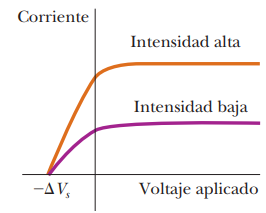
\includegraphics[width = 100px]{corriente_fotoe.png}\\

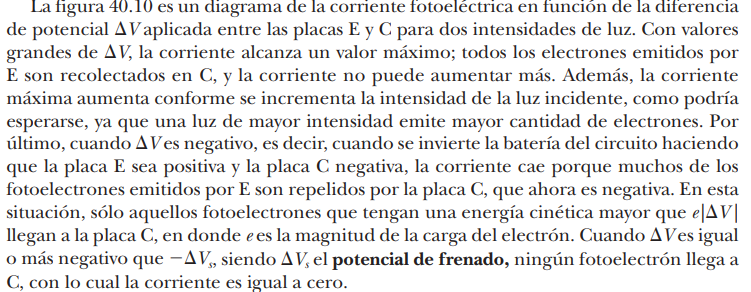
\includegraphics[width = 300px]{corriente_fotoe_explicacion.png}\\

El efecto fotoelectrico tiene 4 caracteristicas que los resultados experimtales no podian explicar:
\begin{itemize}
	\item Dependencia de la energía cinética del fotoelectrón en relación con la intensidad de la luz
	\item Intervalo de tiempo entre la incidencia de la luz y la expulsión de los fotoelectrones.
	\item Dependencia de expulsión de electrones en relación con la frecuencia de la luz.
	\item Dependencia de la energía cinética del fotoelectrón en relación con la frecuencia de la luz.
\end{itemize}

En 1905 Einstein aportó una explicación exitosa del efecto fotoeléctrico y amplió el concepto de cuantización de Planck a las ondas electromagnéticas. Supuso que la luz (o cualquier otra onda electromagnética) de frecuencia ƒ se puede considerar un flujo de cuantos, independientemente de la fuente de la radiación. Hoy en día a esos cuantos les llamamos \textbf{fotones}\\

En el modelo de Einstein del efecto fotoeléctrico, un fotón de la luz incidente transfiere toda su energía hƒ a un electrón particular en el metal. Debido a eso, la absorción de energía por parte de los electrones no es un proceso de absorción continuo, como se asumía en el modelo ondulatorio, sino un proceso discontinuo en el cual la energía es entregada a los electrones en paquetes discretos.\\
Los electrones expulsados de la superficie del metal y que no entran en colisión con otros átomos del metal antes de escapar tienen una energía cinética máxima $K_{max}$. De acuerdo con Einstein, la energía cinética máxima de estos electrones liberados es igual a $K_{max} = hf- \phi$ donde $\phi$  se llama la función trabajo del metal. La función trabajo representa la energía mínima con la cual un electrón está unido en el metal.\\
Con el modelo fotónico de la luz es posible explicar las características observadas del efecto fotoeléctrico que no eran posibles de comprender a partir de los conceptos clásicos.\\

El modelo de Einstein anticipa una correspondencia lineal entre la energía cinética máxima del electrón $K_{max}$ y la frecuencia de la luz $f$.  Se observa dicha correspondencia lineal, como se bosqueja en la figura 40.11, donde la pendiente de las líneas de dicha gráfica $h$ es la constante de Planck. La intersección con el eje horizontal representa la \textbf{frecuencia de corte} por debajo de la cual \textbf{no se emiten electrones}. La frecuencia de corte está relacionada con la función trabajo según la correspondencia $ƒ_c=  \phi/h$. La frecuencia de corte corresponde a la longitud de onda de corte $\lambda_c$ , donde $\lambda_c = \frac{hc}{\phi}$


\paragraph{Efecto Compton}

la teoría ondulatoria clásica de la luz no podía explicar la \textbf{dispersión de los rayos X} a causa los electrones.

Dado que cada electrón se mueve a una rapidez diferente después de la interacción, dependiendo de la cantidad de energía absorbida a causa de las ondas electromagnéticas, la frecuencia de la onda dispersa en un ángulo determinado en relación con la radiación de llegada debe mostrar una distribución de valores con corrimiento Doppler. Contrariamente a esta predicción, los experimentos de Compton demostraron que, en un \textbf{ángulo determinado}, sólo se observa \textbf{una frecuencia de radiación}. Compton y sus colegas se dieron cuenta de que podían explicar estos experimentos si trataban los fotones no como ondas, sino más bien como partículas puntuales de energía $hf$ y con una cantidad de movimiento $hf/c$, y suponiendo que se conserva tanto la energía como la cantidad de movimiento en el sistema aislado del par fotón-electrón en colisión. Compton adoptó un modelo de partícula para algo que era bien conocido como una onda, y hoy por hoy este fenómeno de dispersión es conocido como \textbf{efecto Compton}\\
\linebreak
\textbf{Ecuación de desplazamiento Compton}
\begin{equation*}
	\lambda' - \lambda_0 = \lambda_C(1-cos\theta) \rightarrow \lambda_C = \dfrac{h}{m_e c} = 0.00243nm
\end{equation*}

\textbf{Deducción de la ecuación de desplazamiento Compton}
Es posible deducir la ecuación de corrimiento de Compton si supone que el fotón se comporta como una partícula y entra en colisión elástica con un electrón inicialmente en reposo. Se aplica un modelo de \textbf{sistema aislado} al fotón y al electrón. En el proceso de dispersión, la totalidad de la \textbf{energía} y la \textbf{cantidad de movimiento lineal} del sistema deben \textbf{conservarse}. 


\paragraph{Fotones y ondas electromagnéticas}

La luz se describe en términos de \textbf{fotones} con cierta energía y cantidad de movimiento. También, por otra parte, la luz y otras ondas electromagnéticas exhiben efectos de interferencia y de difracción, que son entendibles sólo mediante una interpretación \textbf{ondulatoria}. ¿Cuál de los modelos es el correcto? La respuesta dependerá del fenómeno que se esté observando.  El resultado final es que necesita aceptar \textbf{ambos modelos} y admitir que no es posible describir la naturaleza verdadera de la luz en función de ninguna concepción clásica única. En otras palabras, el modelo de partícula y el modelo ondulatorio de la luz \textbf{se complementan}.

\paragraph{Propiedades ondulatorias de las partículas}

Louis de \textbf{Broglie} postuló que ya que los fotones tienen a la vez características ondulatorias y de partículas, es posible que \textbf{todas las formas de la materia tengan ambas propiedades}. Según De Broglie, los electrones, justo igual que la luz, tienen una \textbf{naturaleza dual partícula-onda}.\\
\linebreak
\textbf{Longitud de onda de Broglie}
\begin{equation*}
	\lambda = \dfrac{h}{p} = \dfrac{h}{mu}
\end{equation*}

Además, en analogía con los fotones, De Broglie postuló que las partículas obedecen la relación de Einstein E  hƒ, donde E es la energía total de la partícula. En tal caso, la frecuencia de una partícula es

\paragraph{Revisión del experimento de doble rejilla}

un experimento en el que se disparan \textbf{electrones} hacia una \textbf{doble rejilla}. se halla un \textbf{patrón de interferencia} de ondas representativo respecto al conteo por cada minuto, es decir, a la probabilidad de llegada de los electrones. Este patrón de interferencia no debería esperarse si los electrones se comportaran como si fueran partículas clásicas, proporcionando una evidencia clara de que los electrones están interferidos, un comportamiento distinto parecido a la onda. (Sólo se observa el patrón de interferencia si el intervalo de tiempo para la medición es \textbf{suficientemente grande} para que muchos electrones lleguen a la pantalla del detector)\\
\linebreak
Los electrones se detectan como partículas en una mancha localizada sobre la pantalla del detector en algún instante de tiempo, pero la probabilidad de llegada a dicha mancha se determina al encontrar la intensidad de dos ondas que interfieren.\\
\linebreak
sólo se puede decir que el electrón \textbf{pasa a través de ambas rendijas} Sin embargo, a partir del modelo de partícula cuántica, la partícula se puede considerar construida por ondas que existen en \textbf{todo el espacio}. Debido a eso, las componentes ondulatorias del electrón están presentes en ambas rendijas al mismo tiempo, y este modelo conduce a una interpretación más cómoda de este experimento.

\paragraph{El principio de incertidumbre}
Según la mecánica clásica, no existe una barrera básica que impida un refinamiento adicional de los aparatos o de los procedimientos experimentales de medición.Sin embargo, la teoría cuántica dice que básicamente es \textbf{imposible medir}, simultáneas, la \textbf{posición} y la \textbf{cantidad de movimiento} de una partícula con una \textbf{precisión infinita}.\\
\linebreak
\textbf{principio de incertidumbre de Heisenberg} Si se hace una medición con una incertidumbre $\Delta x$ de la posición de una partícula y de manera simultánea se hace una medición con una incertidumbre $\Delta x_p$ de su componente en x de la cantidad de movimiento, el producto de ambas incertidumbres no puede ser nunca menor de

\begin{equation*}
	\Delta x \Delta p_x \geq \dfrac{h}{2}
\end{equation*}

Es decir, físicamente es \textbf{imposible} medir de manera simultánea la \textbf{posición} exacta y la \textbf{cantidad de movimiento} exacto de una partícula. Estas incertidumbres se presentan debido a la \textbf{estructura cuántica} de la materia.\\
\linebreak
Otra forma de expresar este principio es:

\begin{equation*}
	\Delta E \Delta t \geq \dfrac{h}{2}
\end{equation*}

\section{Física atómica}

\paragraph{Espectros atómicos de los gases}

los objetos emiten una radiación térmica, caracterizada por una distribución continua de longitudes de onda. En marcado contraste con este espectro de distribución continua, está el \textbf{espectro de línea} discreto que se observa cuando un gas a \textbf{baja presión} se somete a una \textbf{descarga eléctrica}. La observación y el análisis de estas líneas espectrales se conoce como \textbf{espectroscopia de emisión}. El espectro de línea más \textbf{simple}, que se describe con detalle, es el del átomo de \textbf{hidrógeno}.\\
\linebreak
Otra forma de la espectroscopia, muy útil para analizar sustancias, es la \textbf{espectroscopia de absorción}. Un espectro de absorción se obtiene al pasar una luz blanca de una fuente continua a través de un gas o una solución diluida del elemento que se está analizando.\\
\linebreak
\textbf{Balmer}, descubrió una ecuación empírica que \textbf{predecía} correctamente las \textbf{longitudes de onda} de \textbf{cuatro líneas} de emisión visibles del \textbf{hidrógeno}. Estas eran rojo, azul-verde, azul violeta, y violeta.\\
\linebreak
\textbf{Serie de Balmer}
\begin{equation*}
	\dfrac{1}{\lambda} = R_H \left( \dfrac{1}{2^2}- \dfrac{1}{n^2}  \right) \rightarrow n = 3,4,5,\dots
\end{equation*}

Donde $R_H$ es la \textbf{ constante de Rydberg} con un valor de $1.097 373 2 \times 10^7  m^{-1}$\\
El límite de la serie es la longitud de onda más corta en la serie y corresponde a $n \rightarrow \infty$

\paragraph{Los primeros modelos del átomo}
En 1911, Ernest Rutherford realizó un experimento que demostró que el modelo de Thomson podría no ser correcto. Rutherford explicó sus sorprendentes resultados al desarrollar un nuevo modelo atómico, que suponía que la carga positiva en el átomo estaba concentrada en una región reducida en comparación con el tamaño de éste. Rutherford llamó a esta concentración de carga positiva el \textbf{núcleo} del átomo. todos los electrones pertenecientes al átomo se encuentran en un \textbf{volumen relativamente grande fuera del núcleo}. Para explicar la razón por la cual los electrones \textbf{no son atraídos hacia el núcleo } debido a la fuerza de atracción eléctrica, Rutherford los representó \textbf{moviéndose en órbitas alrededor del núcleo} de la misma forma en que los planetas giran alrededor del Sol

\paragraph{Modelo de Bohr del átomo de hidrógeno}

presentara un nuevo modelo del átomo de hidrógeno que evita las difi cultades del modelo planetario de Rutherford. Bohr combinó las ideas de la teoría cuántica original de Planck, el concepto de Einstein del fotón, el modelo planetario de Rutherford del átomo y la mecánica newtoniana para llegar a un modelo semiclásico en términos de algunos postulados revolucionarios.  Las ideas básicas de la teoría de Bohr, según se aplican al átomo de hidrógeno, son las que siguen
\begin{enumerate}
	\item El electrón se mueve en órbitas circulares alrededor del protón bajo la influencia de fuerza eléctrica de atracción
	\item Sólo ciertas órbitas del electrón son \textbf{estables}. Cuando está en alguno de estos estados \textbf{estacionarios}, como los llamaba Bohr, el electrón \textbf{no emite energía en forma de radiación}. En consecuencia, la energía total del átomo permanece constante y puede utilizarse la mecánica clásica para describir el movimiento del electrón. El modelo de Bohr afirma que el electrón acelerado de manera centrípeta no emite radiación continua, \textbf{perdiendo energía} y finalmente \textbf{girando en los núcleos}
	\item La radiación es emitida por el átomo cuando el electrón hace una \textbf{transición} de una órbita inicial más energética a una órbita de menor energía.  La frecuencia de la radiación emitida se determina por la expresión de la conservación de energía \begin{equation*}
		E_i -E_f = hf
	\end{equation*}
	\item  El tamaño de la órbita permitida del electrón queda determinado por una condición impuesta sobre la cantidad de movimiento angular orbital del electrón: las órbitas permitidas son aquellas para las cuales la cantidad de movimiento angular
orbital del electrón en relación con el núcleo se cuantiza y es igual a un múltiplo entero de $h' = h/2\pi$
\end{enumerate}

La expresión general para el \textbf{radio} de \textbf{cualquier órbita en el átomo de hidrógeno} es:

\begin{equation*}
	r_n = n^2 a_0 = n^2 \cdot (0.052 9 \text{ nm})
\end{equation*}

Siendo $a_0$ el \textbf{radio de Bohr}

La cuantización de los radios de la órbita conduce a la cuantización de la energía. Las energías permitidas del
átomo de hidrógeno de Bohr son:

\begin{equation*}
	E_n = - \dfrac{13.606 \text{ eV}}{n^2} \rightarrow n=1,2,3,\dots
\end{equation*}

las energías del átomo de hidrógeno varían inversamente con $n_2$ , de modo que su \textbf{separación en energía} se vuelve más \textbf{pequeña} conforme $n$ \textbf{aumenta}\\
\linebreak
Las ecuaciones anteriores pueden utilizarse para calcular la \textbf{frecuencia} del fotón emitido cuando el electrón hace una transición de una órbita exterior a una interior.

\begin{equation*}
	f = \dfrac{E_i - E_f}{h} = 
\end{equation*}

Resulta conveniente expresar la ecuación en función de la longitud de onda:

\begin{equation*}
	\dfrac{1}{\lambda} = \dfrac{f}{c} = R_H\left( \dfrac{1}{n_f^2} - \dfrac{1}{n_i^2}\right)
\end{equation*}

\paragraph{Principio de correspondencia de Bohr???}
La física cuántica está de acuerdo con la física clásica cuando la diferencia entre los niveles cuantizados se desvanecen. Este principio, establecido por primera vez por Bohr, se llama principio de correspondencia


\paragraph{Modelo cuántico del átomo de hidrógeno ???}

El número cuántico orbital, simbolizado como , resulta de la ecuación diferencial para f($\theta$) y se asocia con el movimiento angular orbital del electrón. El número cuántico orbital magnético m resulta de la ecuación diferencial para g(f). Tanto  como m son enteros. En la sección 42.6 se amplía el análisis de estos dos números cuánticos y también se presenta un cuarto número cuántico (no entero), resultado de un tratamiento relativístico del átomo de hidrógeno. La aplicación de las condiciones frontera de las tres partes de una función ondulatoria completa lleva a correspondencias importantes entre los tres números cuánticos, como también a ciertas restricciones respecto a sus valores:

\begin{itemize}
	\item Los valores de n son enteros que pueden ir de 1 a $\infty$
	\item Los valores de $l$ son enteros que pueden ir de 0 a $n = -1$
	\item Los valores de $m$ son enteros que pueden ir de $-l $ a $l$
\end{itemize}

\paragraph{Espectros atómicos: Visible y Rayos X}.\\

Recordemos que un átomo \textbf{emite} radiación electromagnética si un electrón en un \textbf{estarlo excitado} hace una transición hacia un estado de \textbf{menor energía}. El conjunto de longitudes de onda observado cuando una especie específica experimenta este tipo de procesos se denomina \textbf{espectro de emisión} para esas especies. De igual modo, los átomos con electrones en la configuración del \textbf{estado base} también pueden \textbf{absorber} radiación electromagnética en longitudes de onda específicas, lo que produce un \textbf{espectro de absorción}. Estos espectros pueden utilizarse para identificar elementos. Cada vez que un electrón efectúa una transición de un estado de energía \textbf{mayor a
uno menor}, se \textbf{emite un fotón} de luz. La frecuencia de este fotón es $f = \Delta E/h$ , donde $\Delta E$ es la diferencia de energía entre los dos niveles. y h es la constante dc Planck. Las reglas de selección para las transiciones permitidas son
\begin{equation*}
	\Delta l = \pm 1
\end{equation*}

Los rayos X se emiten cuando un blanco metálico es \textbf{bombardeado con electrones} de alta energía o cualquier otra partícula cargada. El espectro de rayos X consiste por lo común en una amplia banda continua y en una serie de líneas definidas que dependen del material utilizado para el blanco. Estas líneas se conocen como \textbf{líneas características}

\paragraph{Transiciones atómicas}

Cuando incide radiación sobre un átomo, sólo aquellos fotones cuya energía $hf$ es igual a la energía de separacíon $\Delta E$ entre dos niveles de energía pueden ser absorbidos por el átomo. Este proceso es conocido como \textbf{absorción estimulada} porque el fotón estimula al átomo para realizar la transición hacia un nivel superior.\\
\linebreak
Una vez que el átomo se encuentra en estado excitado, éste puede realizar la transición \textbf{de regreso} hacia un nivel de energía más bajo, \textbf{emitiendo un fotón} en el proceso. Este proceso es conocido como \textbf{emisión espontánea}, porque
sucede naturalmente, sin requerir de un evento que produzca dicha transición. Por lo general, un átomo permanece en un estado excitado durante sólo $10^{-8}$s.\\
\linebreak
Además de la emisión espontánea, también se presenta la \textbf{emisión estimulada} (Durante un atomo en estado exitado \textbf{metaestable} se le incide un foton con una energia  $\Delta E = hf$). después de la emisión estimulada, existen \textbf{dos fotones con energía idéntica} el fotón incidente y el fotón emitido. Los dos están \textbf{en fase} y viajan en la \textbf{misma dirección}

\paragraph{Láser}
Las propiedades principales del láser que lo hacen tan útil para las aplicaciones tecnológicas, son las siguientes
\begin{itemize}
	\item La luz de láser es \textbf{coherente}. Los rayos individuales de luz en un haz láser conservan una correspondencia de fase fija entre sí.
 	\item La luz de láser es \textbf{monocromática}. La luz de un haz láser tiene un intervalo muy limitado de longitudes de onda.
	\item La luz de láser tiene un \textbf{pequeño ángulo de divergencia}. El haz se dispersa muy poco, incluso en grandes distancias.
\end{itemize}

A fi n de que la emisión estimulada dé como resultado una luz láser, debe tener una acumulación de fotones en el sistema. Las tres condiciones siguientes deben ser satisfechas para lograr esta acumulación

\begin{itemize}
	\item El sistema debe estar en un estado de \textbf{inversión de población} (más átomos en un estado
excitado que en el estado base, osea que hay una emision neta de fotones, en vez de una absorsion neta).
	\item El estado excitado del sistema debe ser un estado metaestable, lo que significa que su tiempo
de vida debe ser grande comparado con los usuales tiempos de vida cortos de los estados
excitados. Cuando éste es el caso, la emisión estimulada ocurre antes que la emisión
espontánea.
	\item Los fotones emitidos deben estar confinados en el sistema suficiente tiempo para
permitirles estimular la emisión adicional de otros átomos excitados. 
\end{itemize}

Una de las más inusuales e interesantes aplicaciones del láser es la producción de imágenes
tridimensionales en un proceso llamado \textbf{holografía}.

\end{document}